\cptr{Parameter estimation in nonstandard models}
{Parameter estimation in nonstandard models}
{Dora Matzke, Udo Boehm, and Joachim Vandekerckhove}

\newcommand{\file}[1]{{\texttt{#1}}}
\newcommand{\osf}{\url{https://osf.io/ucmaz/}}

\section{Introduction}
In this special issue, Dienes (this issue) has argued that Bayesian methods are to be preferred over classical methods, Kruschke (this issue) and Etz and Vandekerckhove (this issue) have introduced the Bayesian philosophy and associated mathematics, and Love et al.\ (this issue; see also \citeNP{jasp}) and Wagenmakers et al.\ (this issue) described software that implements standard hypothesis tests within the Bayesian framework. In the present paper, we demonstrate the use of three popular software packages that enable psychologists to estimate parameters in formal models of varying complexity.

The mathematical foundations of Bayesian parameter estimation are not especially difficult---all that is involved are the elementary laws of probability theory to determine the posterior distribution of parameters given the data. Once the posterior distribution has been defined, the final hurdle of Bayesian parameter estimation is to compute descriptive statistics on the posterior. In order to obtain these descriptive statistics, one widely applicable strategy is to draw random samples from the posterior distribution using Markov chain Monte Carlo methods (MCMC; van Ravenzwaaij, this issue)---with sufficient posterior samples, descriptives on the sample set can substitute for actual quantities of interest.

In this article, we describe the use of three popular, general--purpose MCMC engines that facilitate the sampling process. {We will focus on WinBUGS, JAGS, and Stan, and illustrate their use for parameter estimation in two popular models in psychology. The development of these software packages has greatly contributed to the increase in the prevalence of Bayesian methods in psychology over the past decade (e.g., \citeNP{LeeWagenmakersBayesBook}). The packages owe their popularity to their flexibility and usability; they allow researchers to build a large number of models of varying complexity using a relatively small set of sampling statements and deterministic transformations. Moreover, the packages have a smooth learning curve, are well documented, and are supported by a large community of users both within and outside of psychology. Their popularity notwithstanding, WinBUGS, JAGS, and Stan represent only a subclass of the many avenues to Bayesian analysis; the different avenues implement a trade--off between flexibility and accessibility. At one end of the spectrum, researchers may use off--the--shelf Bayesian software packages, such as JASP (Love et al.\ this issue; see also \citeNP{jasp}). JASP has an attractive and user--friendly graphical user interface, but presently it only supports standard hypothesis tests (see also \citeNP{morey2015package}). At the other end of the spectrum, researcher may implement their own MCMC sampler, one that is tailored to the peculiarities of the particular model at hand (e.g., van Ravenzwaaij, this issue; \citeNP{RouderLu2005}). This approach provides tremendous flexibility, but it is time--consuming, labor--intensive, and requires expertise in computational methods. General--purpose MCMC engines---such as WinBUGS, JAGS, and Stan---are the middle--of--the--road alternatives to Bayesian analysis that provide a large degree of flexibility at a relatively low cost.}

{We begin with a short introduction of formal models as generative processes using a simple linear regression as an example. We then show how this model can be implemented in WinBUGS, JAGS, and Stan, with special emphasis on how the packages can be interacted with from R and MATLAB. We then turn to a more complex model, and illustrate the basic steps of Bayesian parameter estimation in a multinomial processing tree model for a false-memory paradigm. The WinBUGS, JAGS, and Stan code for all our examples is available in the Supplemental Materials at \osf{}. The discussion presents a comparison of the strengths and weaknesses of the packages and provides useful references to hierarchical extensions and Bayesian model selection methods using general--purpose MCMC software.} 

\section{An Introduction with Linear Regression}
\subsection{Specification of Models as Generative Processes}

Before we continue, it is useful to consider briefly what we mean by a formal \emph{model}: A formal model is a set of formal statements about how the data come about. Research data are the realizations of some stochastic process, and as such they are draws from some random number generator whose properties are unknown. {In psychology, the random number generator is typically a group of randomly selected humans who participate in a study, and the properties of interest are often differences in group means between conditions or populations (say, the difference in impulsivity between schizophrenia patients and controls) or other invariances and systematic properties of the data generation process.} A formal model is an attempt to emulate the unknown random number generator in terms of a network of basic distributions.

Consider, for example, simple linear regression, with its three basic assumptions of \emph{normality}, \emph{linearity}, and \emph{homoskedasticity}. This common technique implies a stochastic process: the data are assumed to be random draws from a normal distribution (normality), whose mean is a linear function of a predictor (linearity), and whose variance is the same (homoskedasticity) for all units, where ``units'' can refer to participants, items, conditions, and so on. A regression model in which we predict $y$ from $x$ may be written as a follows:
\begin{eqnarray}
y_i | \mu_i, \tau &\sim& \Nor(\mu_i, \tau) \label{eq:reg1}\\
\mu_i |\beta_1, \beta_2, x_i &=&\beta_1 + \beta_2 x_i. \label{eq:reg2}
\end{eqnarray}
The tilde ($\sim$) may be read as ``is a random sample from''. These two statements encode the assumptions of normality (Eq.~\ref{eq:reg1}), homoskedasticity across units $i$ (Eq.~\ref{eq:reg1}), and linearity (Eq.~\ref{eq:reg2}). Usually omitted, but implied, is that these statements hold true for all values that the subscript $i$ can take:
\begin{eqnarray}\forall i, & i=1,\ldots,N.\label{eq:reg3}\end{eqnarray} We use $\tau$ to indicate the \emph{precision}---the inverse of the variance---because that is how WinBUGS and JAGS parameterize the Gaussian distribution.

In the Bayesian framework, we must further specify our prior assumptions regarding the model parameters $\beta_1$, $\beta_2$, and $\tau$. Let us use the following\footnote{We chose values for the parameters of the prior distributions that fit the introductory example. In general, these values should depend on the application at hand (see Vanpaemel \& Lee, this issue; and Morey, this issue).} forms for the priors:
\begin{eqnarray}
\beta_1 &\sim& \Nor(0, 0.001) \label{eq:reg4}\\
\beta_2 &\sim& \Nor(0, 0.001) \label{eq:reg5}\\
\tau    &\sim& \Gamma(0.001,0.001). \label{eq:reg6}
\end{eqnarray}

This simple model also helps to introduce the types of variables that we have at our disposal. Variables can be \emph{stochastic}, meaning that they are draws from some distribution. Stochastic variables can be either observed (i.e., data) or unobserved (i.e., unknown parameters). In this model, $y$, $\beta_1$, $\beta_2$, and $\tau$ are stochastic variables. Variables can also be \emph{deterministic}, which means their values are completely determined by other variables. Here, $\mu_i$ is determined as some combination of $\beta_1$, $\beta_2$, and $x_i$. $N$ is a constant.

{Taken together, a Bayesian model can be thought of as a data--generation mechanism that is conditional on parameters: Bayesian models make \emph{predictions}.
In particular, the \emph{sampling statements}--- including the priors---in Equations~\ref{eq:reg1}, \ref{eq:reg4}, \ref{eq:reg5}, and~\ref{eq:reg6} and the deterministic transformation in Equation~\ref{eq:reg2}, fully define a \emph{generative model}; this set of statements fully defines the model because they are all that is needed to generate data from the model. The generative model thus formalizes the presumed process by which the data in an empirical study were generated.} 

\subsection{A Toy Data Set}
As our introductory example, we will use a small data set containing (a) the observed number of attendees at each session of a recent conference (the data $y$) and (b) the number of attendees that was expected by the organizers (the predictor $x$). Table~\ref{tab:bi3:mpdata} shows the data set.

\lstset{numbers=none}
\begin{table*}[t]
\centering
\caption{Example data set for linear regression. Attendance at each session of a conference, as predicted by the organizers (left) and as observed (middle), with the corresponding ``S--style'' data file (right).}\vspace{1ex}
\begin{tabular}{rr@{\hspace{15pt}}r}
\begin{tabular}{|ccc|}
\multicolumn{3}{c}{Expected ($x$)}\\ \hline
  51 &  24 &  32   \\
  44 &  21 &  42   \\
  57 &  23 &  27   \\
  41 &  28 &  38   \\
  53 &  22 &  32   \\
  56 &  30 &  21   \\
  49 &  29 &  21  \\
  58 &  35 &  12  \\
  50 &  18 &  29  \\
  32 &  25 &  14  \\
  \hline
\end{tabular} & \begin{tabular}{|ccc|}
\multicolumn{3}{c}{Observed ($y$)}\\ \hline
  33 &  35 &  32  \\
  55 &  18 &  31  \\
  49 &  14 &  37  \\
  56 &  31 &  17  \\
  58 &  13 &  11  \\
  61 &  23 &  24  \\
  46 &  15 &  17  \\
  82 &  20 &  \phantom{0}5  \\
  53 &  20 &  16  \\
  33 &  33 &  \phantom{0}7  \\
   \hline
\end{tabular} & \begin{lstlisting}

  x <- c(51, 44, 57, 41, 53, 56,
         49, 58, 50, 32, 24, 21,
         23, 28, 22, 30, 29, 35,
         18, 25, 32, 42, 27, 38,
         32, 21, 21, 12, 29, 14)
  y <- c(33, 55, 49, 56, 58, 61,
         46, 82, 53, 33, 35, 18,
         14, 31, 13, 23, 15, 20,
         20, 33, 32, 31, 37, 17,
         11, 24, 17,  5, 16,  7)
\end{lstlisting}
\end{tabular}\label{tab:bi3:mpdata}
\end{table*}
\vspace{1ex}

\subsection{Implementing a Generative Model}
The generative specification is the core of the BUGS modeling language \cite{LunnEtAl2000} that is used by WinBUGS and dialects of which are used by JAGS and Stan. In all of these programs, the model definition consists of a generative specification. In many cases, the model code is almost a point--to--point translation of a suitable generative specification. Consider this BUGS implementation of the linear regression model:

\begin{lstlisting}
model {
   # linear regression
   for (i in 1:N) {                      # Eq. (*@\ref{eq:reg3}@*)
      y[i] ~ dnorm(mu[i],  tau)          # Eq. (*@\ref{eq:reg1}@*)
      mu[i] <- beta[1] + beta[2] * x[i]  # Eq. (*@\ref{eq:reg2}@*)
   }
   # prior definitions
   beta[1] ~ dnorm(0, 0.001)             # Eq. (*@\ref{eq:reg4}@*)
   beta[2] ~ dnorm(0, 0.001)             # Eq. (*@\ref{eq:reg5}@*)
   tau ~ dgamma(0.001, 0.001)            # Eq. (*@\ref{eq:reg6}@*)
}
\end{lstlisting}

{The parameter \code{beta[1]} denotes the intercept (i.e., observed number of attendees for $0$ expected attendees), \code{beta[2]} denotes the slope of the regression line (i.e., the increase in the observed number of attendees associated with a one--unit increase in the expected number of attendees), and \code{tau} represents the inverse of the error variance.} This short piece of code maps exactly to the generative model for linear regression that we specified. Of course, since there is much more freedom in mathematical expression than there is in computer code, the point--to--point translations will not always be perfect, but it will typically be an excellent starting point. 

In the code, deterministic variables are followed by the \code{<-} assignment operator. For instance, the line \code{mu[i] <- beta[1] + beta[2] * x[i]} specifies that the \code{mu} parameters are given by a linear combination of the of the stochastic \code{beta} variables and the observed data \code{x}. The \code{\#} symbol is used for comments. The complete list of distributions, functions, logical operators, and other programming constructs that are available in WinBUGS, JAGS, and Stan, is listed in their respective user manuals. BUGS is a declarative language, which means that the order of the statements in the model file is largely irrelevant. In contrast, in Stan, the order of statements  matters. With the model translated from formal assumptions to BUGS language, the next step is to interact with the software and sample from the posterior distribution of the parameters.


\section{WinBUGS Graphical User Interface} 

WinBUGS (Bayesian inference Using Gibbs Sampling for Windows; \citeNP{LunnEtAl2000,LunnEtAl2009,SpiegelhalterEtAl2003}; for an introduction see \citeNP{Kruschke2010Book}, \citeNP{LunnEtAl2012}, and \citeNP{LeeWagenmakersBayesBook}) is a stand--alone piece of software that is freely available at \url{http://www.mrc-bsu.cam.ac.uk/bugs/}. In this section we give a brief description of the WinBUGS graphical user interface (GUI) using the linear regression model introduced above; later we illustrate how WinBUGS can be called from other software, such as R and MATLAB. For a detailed step--by--step introduction to the WinBUGS GUI, the reader is referred to \citeA{LeeWagenmakersBayesBook}.

To interact with WinBUGS via the GUI, users have to create a number of files. First, there is a \emph{model file} that describes the generative specification of the model, second is the \emph{data file} that contains the raw data, and third is an \emph{initial values file} that contains some starting values for the sampling run.

Panel~A in Figure~\ref{fig:bi3:GUI1} shows the model file \file{linreg\_model.txt} that describes the generative model for the linear regression example. Panel B shows the data file \file{data.txt}. The data specification follows S-plus object notation, where vectors are encapsulated in the concatenation operator \code{c(...)} and matrices are defined as structures with a dimension field, such as \code{structure(.Data = c(...),.Dim = c(R, C))}, where \code{R} stands for the number of rows and \code{C} for the number of columns. In the linear regression example, the data consist of the vector of observations \code{y} corresponding to the observed number of attendees, a vector of observations \code{x} corresponding to the predicted number of attendees, and a scalar \code{N} corresponding to the number of sessions.

The same data format is used to store the (optional, but strongly recommended) set of initial values for the unobserved stochastic variables. If initial values are not supplied, WinBUGS will generate these automatically by sampling from the prior distribution of the parameters. Automatically generated initial values can provide poor starting points for the sampling run and may result in numerical instability. If multiple MCMC chains are run in order to diagnose convergence problems, we encourage users to create a separate file for each set of initial values. As shown in Panel~C in Figure~\ref{fig:bi3:GUI1}, we will run three chains, each with a different set of initial values, and store these in \file{inits1.txt}, \file{inits2.txt}, and \file{inits3.txt}. 

\begin{figure*}[!htb]
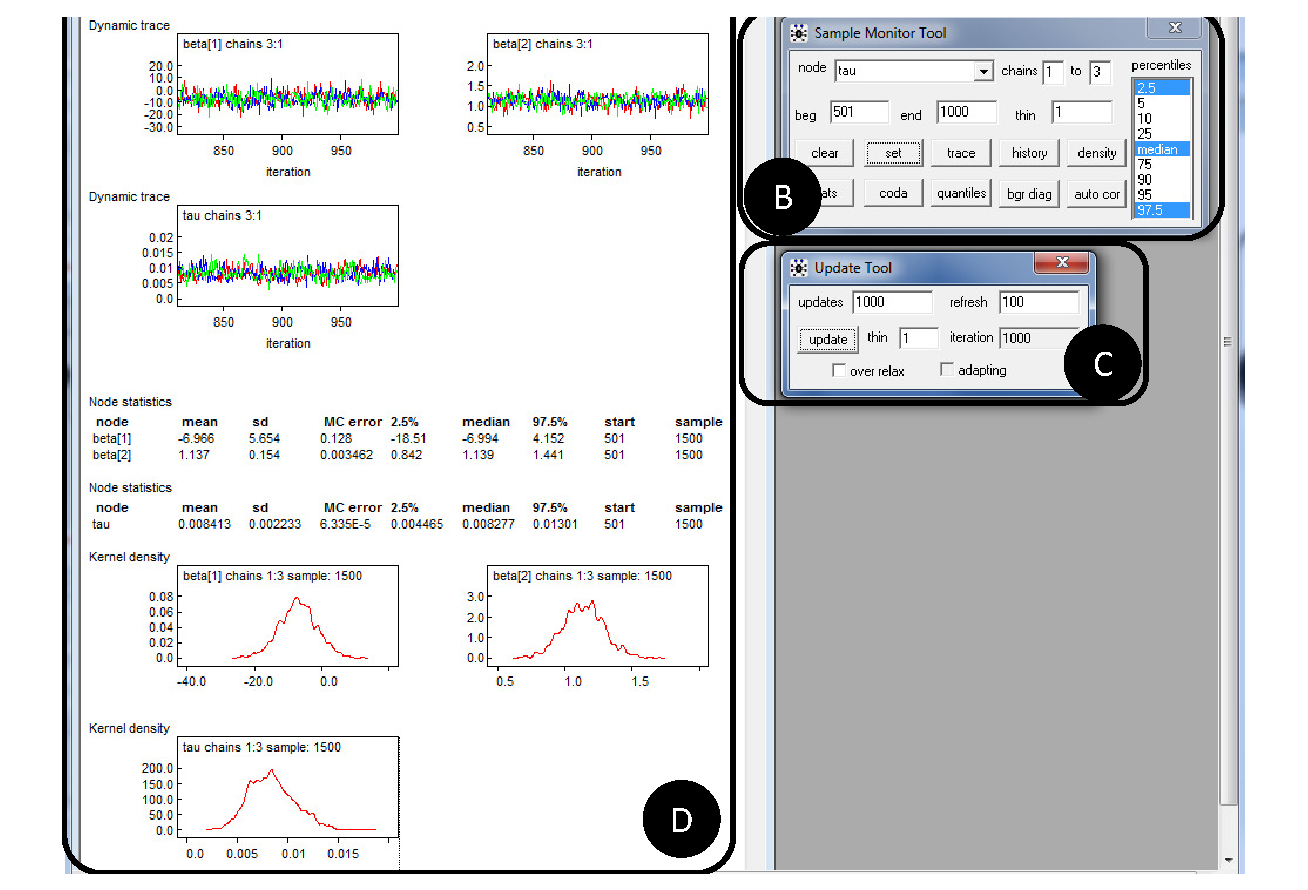
\includegraphics[width=1\textwidth]{figs/bi3_WinBUGS_GUI}
\caption{{The WinBUGS graphical user interface.} Panel~A shows the model file; Panel~B shows the data file; Panel~C shows the initial values; Panel~D shows the Specification Tool window; Panel~E show the status bar.}\label{fig:bi3:GUI1}
\end{figure*} 

Once the model file, the data file, and the files containing the initial values are created, follow the steps outlined below to sample from the posterior distribution of the parameters.

\begin{enumerate}
\item Load the model file and check the model specification. To open the model file, go to \texttt{File -> Open} and select \file{linreg\_model.txt} in the appropriate directory. To check the syntax of the model specification, go to \texttt{Model -> Specification} and open the \texttt{Specification Tool} window (Panel~D in Figure~\ref{fig:bi3:GUI1}), activate the model file by clicking inside \file{linreg\_model.txt}, click on \texttt{check model}, and wait for the message ``model is syntactically correct'' to appear in the status bar.

\item Load the data file. To open the data file, go to \texttt{File -> Open} and select \file{data.txt} in the appropriate directory. To load the data, activate the data file, click on \texttt{load data} in the \texttt{Specification Tool} window, and wait for the message ``data loaded'' to appear in the status bar.

\item Compile the model. To compile the model, specify the number of MCMC chains in the box labeled \texttt{num of chains} in the \texttt{Specification Tool} window, click on \texttt{compile}, and wait for the message ``model compiled'' to appear in the status bar. In the linear regression example, we will run three MCMC chains, so we type ``3'' in the \texttt{num of chains} box.

\item Load the initial values. To open the file that contains the initial values for the first chain, go to \texttt{File -> Open} and select \file{inits1.txt} in the appropriate directory. To load the first set of initial values, activate \file{inits1.txt}, click on \texttt{load inits} in the \texttt{Specification Tool} window, and wait for the message ``chain initialized but other chain(s) contain uninitialized variables''. Repeat these steps to load the initial values for the second and third MCMC chain. After the third set of initial values is loaded, wait for the message ``model is initialized'' to appear in the status bar (Panel~E in Figure~\ref{fig:bi3:GUI1}).

\item Choose the output type. To ensure that WinBUGS pastes all requested output in a single user--friendly log file, go to \texttt{Output -> Output options}, open the \texttt{Output options} window, and select the \texttt{log} option (Panel~A in Figure~\ref{fig:bi3:GUI2}).

\item Specify the parameters of interest. To specify the parameters that you want to draw inference about, go to \texttt{Inference -> Samples}, open the \texttt{Sample Monitor Tool} window, type one by one the name of the parameters in the box labeled \texttt{node}, and click on \texttt{set} (Panel~B in Figure~\ref{fig:bi3:GUI2}). In the linear regression example, we will monitor the \code{beta[1]}, \code{beta[2]}, and \code{tau} parameters. To request dynamic trace plots of the progress of the sampling run, select the name of the parameters in the drop--down menu in the \texttt{Sample Monitor Tool} window and click on \texttt{trace}. WinBUGS will start to display the dynamic trace plots once the sampling has begun. 

\item Specify the number of recorded samples. To specify the number of recorded samples per chain, fill in the boxes labeled \texttt{beg}, \texttt{end}, and \texttt{thin} in the \texttt{Sample Monitor Tool} window. In our linear regression example, we will record $500$ posterior samples for each parameter. We will discard the first $500$ samples as burn--in and start recording samples from the $501^{th}$ iteration (\texttt{beg=501}); we will draw a total of $1,000$ samples (\texttt{end=1000}); and we will record each successive sample without thinning the chains (\texttt{thin=1}).

\item Sample from the posterior distribution of the parameters. To sample from the posteriors, go to \texttt{Model -> Update}, open the \texttt{Update Tool} window (Panel~C in Figure~\ref{fig:bi3:GUI2}), fill in the total number of posterior samples per chain (i.e., $1,000$) in the box labeled \texttt{updates}, specify the degree of thinning (i.e., $1$) in the box labeled \texttt{thin}, click on \texttt{update}, and wait for the message ``model is updating'' to appear in the status bar. 

\item Obtain the results of the sampling run. To obtain summary statistics and kernel density plots of the posterior distributions, select the name of the parameters in the drop-down menu in the \texttt{Sample Monitor Tool} window and click on \texttt{stat} and \texttt{density}. WinBUGS will print all requested output in the log file (Panel~D in Figure~\ref{fig:bi3:GUI2}). {The figures labeled ``Dynamic trace'' show trace plots of the monitored parameters; the three MCMC chains have mixed well and look identical to one another, indicating that the chains have converged to the stationary distribution and that the successive samples are largely independent. The table labeled ``Node statistics'' shows summary statistics of the posterior distribution of the parameters computed based on the sampled values. For each monitored parameter, the table displays the mean, the median, the standard deviation, and the upper-and lower bound of the central $95\%$ credible interval of the posterior distribution. The central tendency of the posterior, such as the mean, can be used as a point estimate for the parameter. This $95\%$ credible interval ranges from the $2.5^{th}$ to the $97.5^{th}$ percentile of the posterior and encompasses a range of values that contains the true value of the parameter with $95\%$ probability; the narrower this $95\%$ credible interval, the more precise the parameter estimate. The figures labeled ``Kernel density'' show density plots of the posterior samples for each parameter.}

\end{enumerate}

\begin{figure*}[!tp]
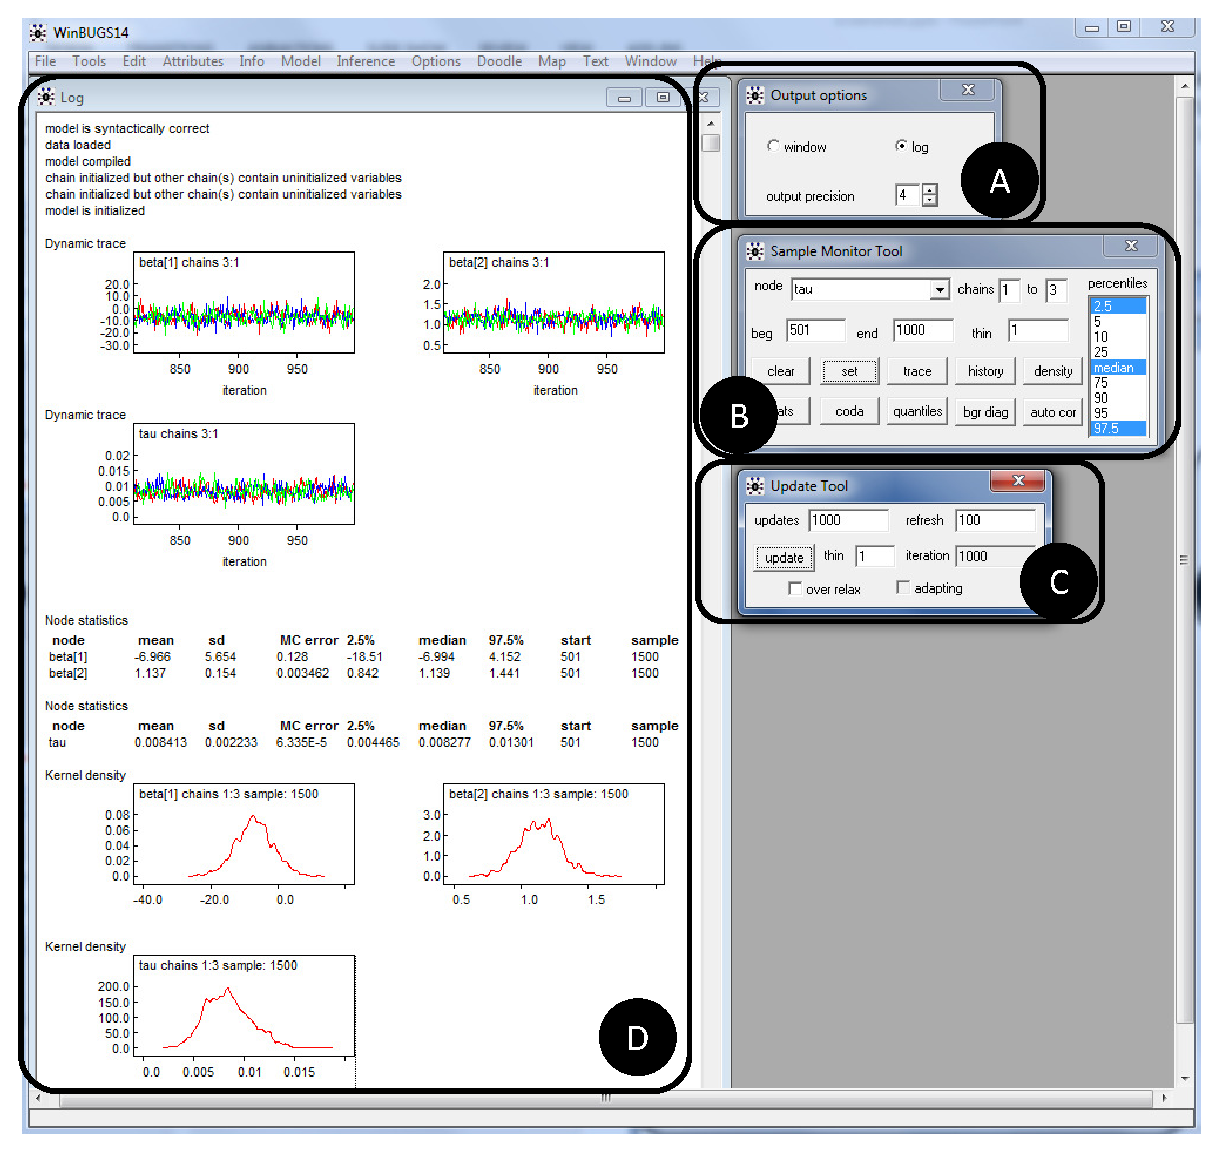
\includegraphics[width=1\textwidth]{figs/bi3_WinBUGS_GUI2}
\caption{{The WinBUGS graphical user interface continued.} Panel~A shows the Output Options window; Panel~B shows the Sample Monitor Tool window; Panel~C shows the Update Tool window; Panel~D shows the log file.}\label{fig:bi3:GUI2}
\end{figure*} 

As the reader might have noticed by now, running analyses via the GUI is inflexible and labor-intensive; the GUI does not allow for data manipulation and visualization and requires users to click through a large number of menus and options. Later we therefore illustrate how WinBUGS can be called from standard statistical software, such as R and MATLAB.


\section{JAGS and Stan Command-Line Interface}
Both JAGS and Stan are based on a command--line interface. Although this type of interface has fallen out of fashion, and it is strictly speaking not required to use either of these programs, we introduce this low-level interface here---using JAGS as the example---in order to provide the reader with an appreciation of the inner workings of other interfaces. Readers who are not interested in this can skip to either one of the next two sections.

Before launching the program, it is again useful to make a set of text files containing the model, data, and initial values. The model file should contain the code in the listing above; for this example, we saved the model in \file{linreg\_model.txt}. 

The data file should contain the data, formatted as in the right column of Table~\ref{tab:bi3:mpdata}. The data format in Table~\ref{tab:bi3:mpdata} is sometimes referred to as ``S--style''; each variable name is given in double quotation marks, followed by the assignment operator \code{<-} and the value to be assigned to the variable. Vectors are encapsulated in the concatenation operator \code{c(...)} and matrices are defined as structures with a dimension field: \code{struct(c(...),.Dim=c(R,C))}, where the $R \times C$ matrix is entered in column--major order. Our data file is called \file{linreg\_data.txt}.

The same data format is used to store the (optional, but strongly recommended) set of initial values. For at least some of the unknowns nodes (i.e., nodes which in the BUGS code are followed by the sampling operator $\sim$), initial values should be provided. If multiple chains will be run, one unique file for each chains is recommended. Our initial values files are called \file{inits1.txt}, \file{inits2.txt}, and \file{inits3.txt}.

Once all these files are in place, start JAGS by opening a command window and typing \code{jags}. Below is the complete interaction with JAGS, in which user input is preceded by the period (\code{.}) prompt. Comments are preceded by a pound sign \code{\#}.

\begin{lstlisting}
~$ jags
Welcome to JAGS 3.4.0 on Mon Jul 20 14:02:50 2015
JAGS is free software and comes with ABSOLUTELY NO WARRANTY
Loading module: basemod: ok
Loading module: bugs: ok
. model in "linreg_model.txt"         # loads the model
. data in "linreg_data.txt"           # loads the data
Reading data file linreg_data.txt
. compile, nchains(3)                 # compiles the model for 3 chains
Compiling model graph
   Resolving undeclared variables
   Allocating nodes
   Graph Size: 117
. parameters in "inits1.txt"          # loads initial values for chain 1
Reading parameter file inits1.init
. parameters in "inits2.txt"          # loads initial values for chain 2
Reading parameter file inits2.txt
. parameters in "inits3.txt"          # loads initial values for chain 3
Reading parameter file inits3.txt
. initialize                          # sets up the sampling algorithms
Initializing model
. update 500                          # draws 500 samples for burn-in
Updating 500
-------------------------------------------------| 500
************************************************** 100%
. monitor set beta, thin(1)           # indicates a variable to save
. monitor set tau, thin(1)            # indicates a variable to save
. update 500                          # draws 500 samples from posterior
Updating 500
-------------------------------------------------| 500
************************************************** 100%
. coda *, stem('samples_')            # saves posterior samples to files
. exit                                # exits
\end{lstlisting}

This will produce a set of files starting with \file{samples\_chain} and an index file starting with \file{samples\_index}. These files can be loaded into a spreadsheet program like Microsoft Excel or LibreOffice Calc (or command line tools like awk and perl) to compute summary statistics and do inference. However, this approach is both tedious and labor--intensive, so there exist convenient interfaces from programming languages such as R, MATLAB, and Python.



\section{Working from MATLAB}

MATLAB is a commercial software package that can be obtained via \url{http://www.mathworks.com/}. Just like Python or R, MATLAB can be used to format data, generate initial values, and visualize and save results of a sampling run. In this section we outline how users can interact with WinBUGS, JAGS, and Stan using MATLAB. R users can skip this section; in the next sections, we will describe how to use R for the same purposes.

To interact with the three computational engines from MATLAB, we will use the Trinity toolbox \cite{vandekerckhovetrinity}, which is developed as a unitary interface to the Bayesian inference engines WinBUGS, JAGS, and Stan. Trinity is a work--in--progress that is (and will remain) freely available via \url{http://tinyurl.com/matlab-trinity}. The MATLAB code needed to call these three engines from Trinity is essentially identical.

To start Trinity, download the toolbox, place it in your MATLAB path, and then call:

\begin{lstlisting}
>> trinity install
>> trinity new
\end{lstlisting}
\noindent The first line will cause the Trinity files to be detected by MATLAB and the second line will create a bare--bones MATLAB script with programming instructions. For example, one line reads:\footnote{It is likely that the exact appearance of this code will vary a little over successive versions of the Trinity toolbox, but the requirements will remain broadly the same.}

\begin{lstlisting}
% Write the model into a variable (cell variable)
model = {
    %$ MODEL GOES HERE $%
    };
\end{lstlisting}
\noindent The user can then enter the model code directly into the MATLAB script, using cell string notation (note the single quotes around each line):

\begin{lstlisting}
model = {
   'model {'
   '   # linear regression'
   '   for (i in 1:N) {'
   '      y[i] ~ dnorm(mu[i], tau)'
   '      mu[i] <- beta[1] + beta[2] * x[i]'
   '   }'
   '   # prior definitions'
   '   beta[1] ~ dnorm(0, 0.001)'
   '   beta[2] ~ dnorm(0, 0.001)'
   '   tau ~ dgamma(0.001, 0.001)'
   '}'
    };
\end{lstlisting}
\noindent It is also possible to write the model in a separate file and provide the file name here instead of the model code. One advantage of writing model code directly into the MATLAB script is that the script can be completely self--contained. Another is that the model code, when treated as a MATLAB variable, could be generated on--the--fly if tedious or repetitive code is required to define a model or if the model file needs to be adapted dynamically (e.g., if variable names need to change from one run to another).

Next, we need to list the parameters of interest (i.e., for which variables we should save posterior samples). For our current application we could list all variables but choose to omit \code{mu} (which is particularly useful if \code{N} is large and the vector \code{mu} takes up much memory):
\begin{lstlisting}
% List all the parameters of interest (cell variable)
params = {
    'beta' 'tau'
    };
\end{lstlisting}

Next, we collect the data variables that MATLAB will send to the computational engine. Again, it is possible to do this by providing the name to a properly formatted data file, but it is more practical to make a MATLAB variable that contains the data. To collect the data, make a \emph{structure variable} as follows (for the example, \code{x} and \code{y} should first be defined with the values given in Table~\ref{tab:bi3:mpdata}):

\begin{lstlisting}
% Make a structure with the data (note that the name of the field needs to
% match the name of the variable in the model)
data = struct(...
    'x', x, ...
    'y', y, ...
    'N', numel(x) ...
    );
\end{lstlisting}
Each field name (in single quotes) is the name of the variable as it is used in the model definition.\footnote{Because MATLAB does not differentiate between vectors and single--column or single--row matrices, but some of the computational engines do, it is sometimes convenient to pass variables explicitly as a matrix or explicitly as a vector. For this situation, Trinity allows the flags \code{AS\_MATRIX\_} and \code{AS\_VECTOR\_} to be prepended to any variable name. A common situation in which this is useful is when matrix multiplication is applied in the model, but one of the matrices has only one column. JAGS, for example, will treat that matrix as a vector and throw a ``dimension mismatch'' error unless the flag is applied. In our example, the data structure would then be defined as \code{struct('AS\_MATRIX\_x', x)}.} Note that Trinity will not permit the model code to have variable names containing underscores, as this symbol is reserved for internal use. Following each field name is the value that this variable will take; this value is taken from the MATLAB workspace, so it can be an existing variable with any name, or it can be a MATLAB expression that generates the correct value, as we did here with \code{N}. Of course, before making this data structure, the data may need to be parsed, read into MATLAB, and possibly pre--processed (outliers removed, etc.).

The final block to complete is a little more involved and requires understanding of MATLAB's \emph{anonymous functions} construct. Anonymous functions are in--line function definitions that are saved as variables. A typical command to define an anonymous function has the following structure:

\begin{center}
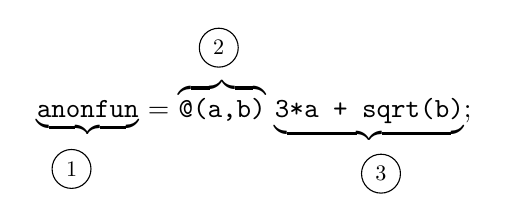
\begin{tikzpicture}[xscale=1,yscale=1]
\tikzstyle{node}=[circle,scale=0.8,draw]
\node[node] at (-0.45,1.80) {2};
\node[] at (0,1) {${\underbrace{\mbox{\texttt{anonfun}}}}$ = $\overbrace{\mbox{\texttt{@(a,b)}}}$ $\underbrace{\mbox{\texttt{3*a + sqrt(b)}}}$;};
\node[node] at ( 1.61,0.20) {3};
\node[node] at (-2.32,0.26) {1};
\end{tikzpicture}
\end{center}
\noindent In this example, \code{anonfun} (part~(1)) is the name given to the new function---this can be anything that is a valid MATLAB variable name. Part~{(2)} indicates the start of an anonymous function with the \code{@} symbol and lists the input variables of the function between parentheses. Part~{(3)} is a single MATLAB expression that returns the output variable, computed from inputs \code{a} and \code{b}. This anonymous function could be invoked with: \code{anonfun(1,4)}, which would yield $5$.

It is possible for an anonymous function to take no (zero) input arguments. For example, \code{nrand = @()-rand} will create a function called \code{nrand} that generates uniformly distributed variates between $-1$ and $0$. In order to supply the computational engine with initial values for the sampling process, we will define an anonymous function that draws a sample from the prior distribution of all or part of the parameter set. An example is:

\begin{lstlisting}
% Write a function that generates a structure with one random value for
% each parameter in a field
generator = @()struct(... 
    'beta' , randn(2, 1) * 10 + 0, ...
    'tau'  , rand * 5 ...
    );
\end{lstlisting}
\noindent Here, a structure is generated with one field for each parameter, and a random initial value for each. The initial value for each of the two \code{beta}s is generated from a normal distribution with mean 0 and standard deviation 10, and \code{tau} is generated from a uniform distribution between 0 and 5. The function \code{generator()} can now be called from MATLAB:

\begin{lstlisting}
>> generator()
ans = 
    beta: [2x1 double]
    tau: 0.6349
\end{lstlisting}
\noindent Note that either of these variables can be validly omitted, but at least one must be given. If one of the random number generators draws a value that is not allowed by the model (e.g., where the prior or likelihood is zero), the engines will throw errors (e.g., JAGS will call them ``invalid parent values''). If no initial values are given, both the engine and Trinity will proceed without error, \emph{but in some engines all MCMC chains will have the same starting point}, rendering any convergence statistics invalid. It is always prudent to provide at least some initial values. Initial values can be scalars, vectors, or matrices, as needed.

Once all of these variables are prepared, they can be handed off to the main function of Trinity, \code{callbayes}. This function can take a large number of input fields to control the behavior of the engine, which can be WinBUGS, JAGS, or Stan (WinBUGS is currently limited to Windows operating systems, and Stan is limited to unix--based systems). To select the computational engine, set \code{engine} to \code{'bugs'}, \code{'jags'}, or \code{'stan'}. (Note that if Stan is selected, the model code should be changed to the Stan code provided in the next section.) More detail regarding the use of \code{callbayes} can be found in its help documentation (\code{doc callbayes}). These default inputs are generally sufficient:

\lstset{numbers=left}
\begin{lstlisting}
[stats, chains, diagnostics, info] = callbayes(engine, ...         (*@\label{line:01}@*)
    'model'          ,     model , ...   % the model as a cell     (*@\label{line:02}@*)
    'data'           ,      data , ...   % the data as a struct    (*@\label{line:03}@*)
    'outputname'     , 'samples' , ...   % any character string    (*@\label{line:04}@*)
    'init'           , generator , ...   % an anonymous function   (*@\label{line:05}@*)
    'datafilename'   ,   proj_id , ...   % any character string    (*@\label{line:07}@*)
    'initfilename'   ,   proj_id , ...   % any character string    (*@\label{line:08}@*)
    'scriptfilename' ,   proj_id , ...   % any character string    (*@\label{line:09}@*)
    'logfilename'    ,   proj_id , ...   % any character string    (*@\label{line:10}@*)
    'nchains'        ,        3  , ...   % the number of chains    (*@\label{line:11}@*)
    'nburnin'        ,     1000  , ...   % the burnin period       (*@\label{line:12}@*)
    'nsamples'       ,    10000  , ...   % how many saved samples? (*@\label{line:13}@*)
    'monitorparams'  ,    params , ...   % the cell string         (*@\label{line:14}@*)
    'thin'           ,        1  , ...   % the thinning factor     (*@\label{line:15}@*)
    'workingdir'     ,    ['/tmp/' proj_id]  , ...   % a temp dir  (*@\label{line:16}@*)
    'verbosity'      ,        0  , ...   % higher is more verbose  (*@\label{line:17}@*)
    'saveoutput'     ,     true  , ...   % save JAGS log file?     (*@\label{line:18}@*)
    'parallel'       ,    false  , ...   % use multiple cores?     (*@\label{line:19}@*)
    'modules'        ,  {'dic'}  );      % use extra modules?      (*@\label{line:20}@*)
\end{lstlisting}
\lstset{numbers=none}

Often, many of these settings can be omitted, and Trinity will choose default values that are appropriate for the engine and operating system. The first input selects the engine. The various \code{'*filename'} inputs on lines~\ref{line:07}--\ref{line:10} serve to organize the temporary files in a readable fashion, so that the user can easily access them for debugging or reproduction purposes.\footnote{When using JAGS or Stan, the working directory will contain a file with a cryptic name that starts with \texttt{tp} and ends in a sequence of random characters, with no file extension. This is the entry point script that Trinity uses to call the engine. It can be used to reproduce the analysis outside of MATLAB, if desired---the files in that directory that do not have the \file{.txt} extension are all that is needed for reproduction. The \file{*.txt} files are output, containing the posterior samples and the log file. When using WinBUGS, data files, initial values files, and model files will be available in the working directory where they can be accessed with the WinBUGS GUI.}

The input values on lines~\ref{line:11}--\ref{line:15} determine how many independent chains should be run, how many samples should be used for burn--in, how many samples should be saved per chain, which parameters should be saved, and by how much the chains should be thinned ($n$ means every $n^{th}$ sample is saved). Line~\ref{line:16} determines a working directory, which is currently set to a value that will work well on unix systems; Windows users might want to change this. Line~\ref{line:17} determines how much output Trinity gives while it is running. Line~\ref{line:18} decides whether the text output given by the engine should be saved.

Line~\ref{line:19} determines if parallel processing should be used---if this is set to \code{true}, all the chains requested on line~\ref{line:11} will be started simultaneously.\footnote{On unix systems, this requires the installation of the free program GNU parallel \cite{Tange2011a}. On Windows systems, it currently requires the MATLAB Parallel Computing Toolbox, but we are working to resolve this dependency.} Note that for complex models, this may cause computers to become overburdened as all the processing power is used up by Trinity. Users who want to run multiple chains than they have computing cores available can use the optional input pair \code{'numcores', C, ...}, where \code{C} is the maximum number of cores Trinity is allowed to use. Finally, line~\ref{line:20} lists optional extra modules (JAGS only). By default, the \code{dic} module is called because this facilitates tracking of the model deviance as a variable. Users with programming experience can create their own modules for inclusion here \cite<e.g., \code{'wiener'}; see>{wabersich2014extending}.

A successful \code{callbayes} call will yield up to four output arguments. \code{stats} contains summary statistics for each saved parameter (mean, median, standard deviation, and the mass of the posterior below 0). These can be used for easy access to parameter estimates. \code{chains} contains all the posterior samples saved. The usefulness of this is discussed below. \code{diagnostics} provides quick access to the convergence metric $\hat{R}$ and the number of effective samples \cite{GelmanRubin1999}. \code{info} gives some more information, in particular the model variable and a list of all the options that were set for the analysis (combining the user--provided and automatically generated settings).

The most important output variable is \code{chains}, which contains the saved posterior samples that are the immediate goal of the MCMC procedure. This variable is used by practically all functions in Trinity that do post--processing, summary, and visualization. The default Trinity script contains the line \code{grtable(chains, 1.05)}. The \code{grtable} function prints a table with a quick overview of the sampling results, such as the posterior mean, the number of samples drawn, the number of effective samples (\code{n\_eff}) and the $\hat{R}$ convergence metric. The second input to \code{grtable} can be either a number, in which case only parameters which an $\hat{R}$ larger than that number will be printed (or a message that no such parameters exist); or it can be a string with a \emph{regular expression}, in which case only parameters fitting that pattern will be shown.\footnote{Regular expressions are an extremely powerful and flexible programming constructs. To give some examples: if the expression is \code{'beta'}, all parameters with the string \code{beta} in their name will be shown. If it is \code{'\textasciicircum{}beta'}, only parameters starting with that string will be shown. \code{'beta\$'} will show only those ending in that string. \code{'.'} will match any variable, and \code{'be|ta'} will match anything containing \code{be} \emph{or} \code{ta}. A complete overview to regular expressions in MATLAB can be found via the documentation for the function \code{regexp}.} 

Another useful function that relies on the \code{chains} variable and on regular expressions is \code{codatable}, which prints a table with user--selected statistics for selected parameters. For example, to see the posterior mean and standard deviation of the \code{beta} parameters:
\begin{lstlisting}
>> codatable(chains, 'beta', @mean, @std)
  Estimand        mean         std
    beta_1      -6.937       5.624
    beta_2       1.139      0.1554
\end{lstlisting}
Finally, Trinity contains a set of functions for visualizing MCMC chains and posterior distributions, but for the present application, a simple scatter plot and regression line suffice (Figure~\ref{fig:bi3:linreg}):
\begin{lstlisting}
scatter(x, y)
line(xlim, stats.mean.beta_1 + stats.mean.beta_2 * xlim)
\end{lstlisting}
\noindent Note that the posterior distributions of the regression parameters contain the first bisector ($\beta_1 \approx 0$, $\beta_2 \approx 1$).

\begin{figure*}[bt]
  \begin{center}
    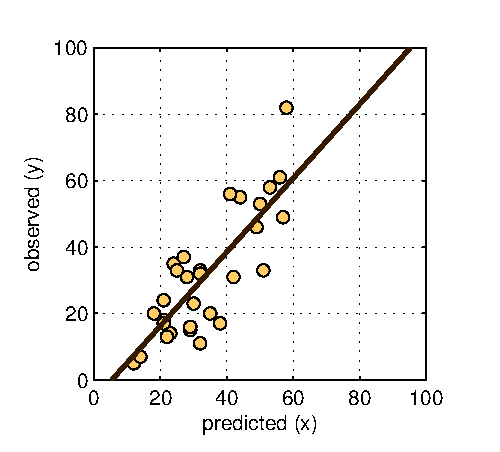
\includegraphics{figs/bi3_linreg.eps}
    \caption{Results of the linear regression example. The best fitting regression line is very close to the first bisector $y=x$.} \label{fig:bi3:linreg}
  \end{center}
\end{figure*}



\section{Working from R}

R \cite{R} is a free statistical software package that can be downloaded from \url{http://www.r-project.org/}. In this section, we outline how users can interact with WinBUGS, JAGS, and Stan using R. As with MATLAB, using R to run analyses increases flexibility compared to working with these Bayesian engines directly; users can use R to format the data, generate the initial values, and visualize and save the results of the sampling run using simple R commands.

\subsection{Interacting with WinBUGS: R2WinBUGS}

To interact with WinBUGS, users have to install the \code{R2WinBUGS} package \cite{SturtzEtAl2005}. The \code{R2WinBUGS} package allows users to call WinBUGS from within R and pass on the model specification, the data, and the initial values to WinBUGS using the \code{bugs()} function. WinBUGS then samples from the posterior distribution of the parameters and returns the MCMC samples to R. 

The following R code can be used to sample from the posterior distribution of the model parameters in the linear regression example using WinBUGS. 

\begin{lstlisting}
# set working directory
setwd("C:/Dropbox/My Documents/Bayesian_estimation/WinBUGS")
# load R2WinBUGS package
library(R2WinBUGS)
\end{lstlisting}

\noindent The \code{setwd()} function specifies the working directory where R will look for the model file and will save the results. The \code{library()} function loads the \code{R2WinBUGS} package.

\begin{lstlisting}
# create vector that contains the expected number of attendees
x <- c(51, 44, 57, 41, 53, 56, 49, 58, 50, 32,
       24, 21, 23, 28, 22, 30, 29, 35, 18, 25,
       32, 42, 27, 38, 32, 21, 21, 12, 29, 14)
# create vector that contains the observed number of attendees
y <- c(33, 55, 49, 56, 58, 61, 46, 82, 53, 33,
       35, 18, 14, 31, 13, 23, 15, 20, 20, 33,
       32, 31, 37, 17, 11, 24, 17,  5, 16,  7)
# create a scalar that contains the number of sessions
N <- 30
# create a list that contains the data and will be passed on to WinBUGS
mydata <- list("y", "x", "N") 
\end{lstlisting}

\noindent Here we create a list named \code{mydata} that contains the data (i.e., \code{x}, \code{y}, and \code{N}) and will be passed on to WinBUGS.

\begin{lstlisting}
# create the initial values for the unobserved stochastic nodes 
myinits=function(){
    list(beta=rnorm(2, 0, 10), tau=runif(1, 0, 5))
}
\end{lstlisting}

\noindent Here we create the initial values for the unobserved stochastic nodes. The initial values for \code{beta[1]} and \code{beta[2]} are random deviates from a zero--centered normal distribution with a standard deviation of $10$ generated using the \code{rnorm()} function. The initial values for \code{tau} are generated from a uniform distribution with lower bound of $0$ and upper bound of $5$ using the \code{runif()} function.
The code generates a unique set of initial values for each chain.

\begin{lstlisting}
# specify parameters of interest	
myparameters <- c("beta", "tau")
\end{lstlisting}

\noindent Here we create a vector that contains the names of the model parameters that we want to draw inference about.  

\begin{lstlisting}
# call WinBUGS
samples <- bugs(data=mydata, inits=myinits, parameters=myparameters,
    model.file="linreg_model.txt", n.chains=3, n.iter=1000, n.burnin=500, 
    n.thin=1, DIC=FALSE, bugs.directory="C:/WinBUGS14", codaPkg=FALSE,
    debug=FALSE)
\end{lstlisting}

\noindent The \code{bugs()} function calls WinBUGS and passes on the model specification, the data, and the start values using the following arguments:
\begin{itemize}
\item \code{data} specifies the list object that contains the data.
\item \code{inits} specifies the list object that contains the initial values.
\item \code{parameters} specifies the vector that lists the names of the parameters of interest.
\item \code{model.file} specifies the text file that contains the model specification. The \code{model.file} argument can also refer to an R function that contains the model specification that is written to a temporary file.
\item \code{n.chain} specifies the number of MCMC chains.
\item \code{n.iter} specifies the total number of samples per chain.
\item \code{n.burnin} specifies the number of samples per chain that will be discarded at the beginning of the sampling run.
\item \code{n.thin} specifies the degree of thinning.
\item \code{DIC} specifies whether WinBUGS should return the Deviance Information Criterion (DIC; \citeNP{SpiegelhalterEtAl2002}) measure of model comparison. 
\item \code{bugs.directory} specifies the location of \texttt{WinBUGS14.exe}.
\item \code{codaPkg} specifies the output that is returned from WinBUGS. Here \code{codaPkg} is set to \code{FALSE} to ensure that
WinBUGS returns the posterior samples in the \code{samples} object. If \code{codaPkg} is set to \code{TRUE}, WinBUGS returns the paths to a set of files that contains the WinBUGS output.  
\item \code{debug} specifies whether WinBUGS will be automatically shut down after sampling. Here \code{debug} is set to \code{FALSE} to ensure that WinBUGS shuts down immediately after sampling and returns the results to R. If \code{debug} is set to \code{TRUE}, WinBUGS will not shut down after sampling and will display summary statistics and trace plots of the monitored parameters. As the name suggests, setting \code{debug} to \code{TRUE} can also provide---often cryptic---cues for debugging purposes.
\end{itemize}

\noindent For more details on the use of \code{bugs()}, the reader is referred to the help documentation. 

Once WinBUGS has finished sampling, it returns the posterior samples to R in the \code{samples} object. The results of the sampling run can be accessed, visualized, and summarized using, for instance, the following code: 

\begin{lstlisting}
# display the first 15 samples in the first chain for tau
samples$sims.array[1:15,1,"tau"]
# plot a histogram of the posterior distribution of tau
hist(samples$sims.array[,,"tau"])
# display summary statistics of the posterior distributions
print(samples) 
\end{lstlisting}

\noindent The posterior samples for $\code{beta[1]}$, $\code{beta[2]}$, and $\code{tau}$ are stored in \code{samples\$sims.array} (or \code{samples\$sims.list}). The \code{hist()} function can be used to plot histograms of the posterior distribution of the parameters based on the samples values. The \code{print(samples)} command displays a useful summary of the posterior distribution of each model parameter, including the mean, the standard deviation, and the quantiles of the posteriors, and (if multiple chains are run) the $\hat{R}$ convergence metric.



\subsection{Interacting with JAGS: R2jags}

To interact with JAGS, users have to install the \code{R2jags} package \cite{su2012r2jags}. The \code{R2jags} package allows users to call JAGS from within R and pass on the model specification, the data, and the start values to JAGS using the \code{jags()} function. JAGS then samples from the posterior distribution of the parameters and returns the MCMC samples to R. 

The R code for running the MCMC routine for the linear regression example in JAGS is similar to the R code for running the WinBUGS analysis outlined in the previous section, with the following modifications. Instead of loading the \code{R2WinBUGS} package, load the \code{R2jags} package by typing:
\begin{lstlisting}
# load R2jags
library(R2jags)
\end{lstlisting}

\noindent Once the \code{mydata}, \code{myinits}, and \code{myparameters} objects are created in R, use the \code{jags()} function to call JAGS and sample from the posterior distribution of the parameters:

\begin{lstlisting}
# call JAGS
samples <- jags(data=mydata, inits=myinits,
    parameters.to.save=myparameters, model.file="linreg_model.txt", 
    n.chains=3, n.iter=1000, n.burnin=500, n.thin=1, DIC=FALSE)
\end{lstlisting}

\noindent The \code{jags()} function takes as input the following arguments:
\begin{itemize}
\item \code{data} specifies the list object that contains the data.
\item \code{inits} specifies the list object that contains the initial values.
\item \code{parameters.to.save} specifies the vector that lists the names of the parameters of interest.
\item \code{model.file} specifies the file that contains the model specification. The \code{model.file} argument can also refer to an R function that contains the model specification that is written to a temporary file.
\item \code{n.chains} specifies the number of MCMC chains.
\item \code{n.iter} specifies the total number of samples per chain.
\item \code{n.burnin} specifies the number of samples per chain that will be discarded at the beginning of the sampling run.
\item \code{n.thin} specifies the degree of thinning.
\item \code{DIC} specifies whether JAGS should return the DIC. 
\end{itemize}

\noindent For more details on the use of \code{jags()}, the reader is referred to the help documentation. 

Once JAGS has finished sampling, it returns the posterior samples to R in the \code{samples} object. The results of the sampling run can be accessed, visualized, and summarized using, for instance, the following code: 

\begin{lstlisting}
# display the first 15 samples in the first chain for tau
samples$BUGSoutput$sims.array[1:15,1,"tau"]
# plot a histogram of the posterior distribution of tau
hist(samples$BUGSoutput$sims.array[,,"tau"])
# display summary statistics of the posterior distributions
print(samples)
# plot traceplot; press ENTER for page change
traceplot(samples)
\end{lstlisting}

\noindent The posterior samples for $\texttt{beta[1]}$, $\texttt{beta[2]}$, and $\texttt{tau}$ are stored in \code{samples\$BUGSoutput\$sims.array} (or \code{samples\$BUGSoutput\$sims.list}), and can be visualized and summarized using the \code{hist()} and \code{print()} functions, respectively. As the name suggests, the \code{traceplot(samples)} command displays trace plots of the model parameters, which provide useful visual aids for convergence diagnostics.



\subsection{Interacting with Stan: rstan}
To interface R to Stan, users need to install the \code{rstan} package \cite{Guo2015rstan}. The \code{rstan} package allows users to call Stan from within R and pass the model specification, data, and starting values to Stan using the \code{stan()} function. The MCMC samples from the posterior distribution generated by Stan are then returned and can be further processed in R.

There are a few differences between WinBUGS/JAGS and Stan that are worth noting when specifying Stan models. While JAGS and WinBUGS simply interpret the commands given in the model, Stan compiles the model specification to a \code{C++} program. Consequently, Stan differentiates between a number of different variable types, and variables in a model need to be declared before they can be manipulated. Moreover, model code in Stan is split into a number of blocks, such as \emph{``data''} and \emph{``model''}, each of which serves a specific purpose. Finally, unlike in WinBUGS and JAGS, the order of statements in a Stan model matters and statements cannot be interchanged with complete liberty.

To run the R code for the linear regression example in Stan, begin by loading the \code{rstan} package:

\begin{lstlisting}
# load rstan package
library(rstan)
\end{lstlisting}

\noindent The \code{mydata}, \code{myinits}, and \code{myparameters} are created in R as illustrated before. However, as Stan relies on a somewhat different syntax than WinBUGS and JAGS, we need to rewrite the model file so it can be parsed by Stan. Here we chose to specify the Stan model as a vector string in R and pass it directly to Stan's sampling function. Note, however, that we could get the same result by simply saving the code as, say, \file{linreg\_model.stan}.

\begin{lstlisting}
# specify Stan model as a string vector
linreg_model <- "data{
    int<lower=1> N;
    vector[N]    x;
    vector[N]    y;
}
parameters{
    vector[2]     beta;
    real<lower=0> sigma2;
}
transformed parameters{
    real<lower=0>  tau;
    tau <- pow(sigma2, -1);
	
    real<lower=0>  sigma;
    sigma <- pow(sigma2, 0.5);
}
model{
    // prior definitions
    beta[1] ~ normal(0, sqrt(1000));                           // Eq. (*@\ref{eq:reg4}@*)
    beta[2] ~ normal(0, sqrt(1000));                           // Eq. (*@\ref{eq:reg5}@*)
    // inverse gamma prior for the variance
    sigma2 ~ inv_gamma(0.001, 0.001)                           // Eq. (*@\ref{eq:reg6}@*)
    // linear regression
    for(i in 1:N){                                             // Eq. (*@\ref{eq:reg3}@*)
        y[i] ~ normal(beta[1] + beta[2] * x[i], sigma);        // Eqs. (*@\ref{eq:reg1}@*)-(*@\ref{eq:reg2}@*)
    }
}"
\end{lstlisting}
\noindent There are a number of very obvious ways in which this model specification differs from that in WinBUGS and JAGS. The model code is split into four blocks and all variables that are mentioned in the ``model'' block are defined in the preceding blocks. The ``data'' block contains the definition of all observed data that are provided by the user. The ``parameters'' block contains the definition of all stochastic variables, and the ``transformed parameters'' block contains the definition of all transformations of the stochastic variables. The difference between these latter two parts of the code is rather subtle and has to do with the number of times each variable is evaluated during the MCMC sampling process; a more elaborate explanation can be found in the Stan reference manual \cite{StanMan}.

We will not discuss the specifics of all the variable definitions here (see \citeNP{StanMan}, for details) but will rather illustrate a few important points using as example the $\code{tau}$ variable. As in the model specification for WinBUGS and JAGS, $\code{tau}$ is the precision of the Gaussian distribution. Defining a variable for the precision of the Gaussian is, strictly speaking, not necessary because distribution functions in Stan are parameterized in terms of their standard deviation. Nevertheless, we retain $\code{tau}$ for easy comparability of the Stan MCMC samples with the output of WinBUGS or JAGS. The first line of the definition of $\code{tau}$ states that it is a real number that is not smaller than 0, and Stan will return an error message should it encounter a negative value for $\code{tau}$ during the sampling process. The next line states that \code{tau} is the inverse of the variance of the Gaussian. If we were to reverse the order of these last two lines, due to Stan's line--by--line evaluation of the code, we would get an error message stating that the variable $\code{tau}$ is not defined.

The specification of the actual sampling statements in the ``model'' block begins, in line with Stan's line--by--line evaluation style, with the prior distributions for the regression coefficients $\code{beta[1]}$ and $\code{beta[2]}$ and the variance of the Gaussian. Note that the prior for $\code{sigma2}$ is an inverse gamma distribution%
---this is equivalent to the prior specification in the WinBUGS/JAGS model where the inverse of the variance was given a gamma prior. Finally, we summarized equations \ref{eq:reg1} and \ref{eq:reg2} into a single line, which is another way in which the Stan model specification differs from the WinBUGS/JAGS code. While WinBUGS does not allow users to nest statements within the definition of a stochastic node, Stan (and also JAGS) users can directly specify the mean of the Gaussian to be a function of the regression coefficients and observed data $\code{x}$, without needing to define $\code{mu[i]}$.

To sample from the posterior distribution of the parameters, call the \code{stan()} function:

\begin{lstlisting}
# call Stan
samples <- stan(data = mydata, init = myinits, pars = myparameters,
    model_code = linreg_model,
    chains = 3, iter = 1000, warmup = 500, thin = 1)
\end{lstlisting}

\noindent The \code{stan()} function takes as input the following arguments:
\begin{itemize}
\item \code{data} specifies the list object that contains the data.
\item \code{init} specifies the list object that contains the initial values.
\item \code{pars} specifies the vector that lists the names of the parameters of interest.
\item \code{model\_code} specifies the string vector that contains the model specification. Alternatively, the name of a \code{.stan} file that contains the model specification can be passed to Stan using the \code{file} argument.
\item \code{chains} specifies the number of MCMC chains.
\item \code{iter} specifies the total number of samples per chain.
\item \code{warmup} specifies the number of samples per chain that will be discarded at the beginning of the sampling run.
\item \code{thin} specifies the degree of thinning.
\end{itemize}

\noindent For more details on the use of \code{stan()}, we refer readers to the corresponding R help file.

Once sampling is finished, Stan returns the posterior samples to R in the \code{samples} object. The results of the sampling run can be accessed, visualized, and summarized using the following code:

\begin{lstlisting}
# display the first 15 samples for tau
extract(samples, pars="tau", inc_warmup=F)$tau[1:15]
\end{lstlisting}

\noindent The posterior samples in the \code{samples} object can most easily be accessed using the \code{extract()} function, which takes as input arguments:
\begin{itemize}
\item \code{samples} object containing the posterior samples from Stan.
\item \code{pars} character vector with the names of the parameters for which the posterior samples should be accessed.
\item \code{inc\_warmup} logical value indicating whether warm--up samples should be extracted too.
\end{itemize}

\begin{lstlisting}
# plot a histogram of the posterior distribution of tau
hist(extract(samples, pars="tau")$tau)
# display summary statistics of the posterior distributions
print(samples)
# plot traceplot; press ENTER for page change
traceplot(samples)
\end{lstlisting}

\noindent The posterior samples for $\texttt{beta[1]}$, $\texttt{beta[2]}$, and $\texttt{tau}$ can be visualized and summarized using the \code{hist()} and \code{print()} functions, respectively. As the name suggests, the \code{traceplot(samples)} command displays trace plots of the model parameters, which provide useful visual aids for convergence diagnostics.



\section{Example: Multinomial Processing Tree for Modeling False--Memory Data}

{In this section, we illustrate the use of WinBUGS, JAGS, and Stan for Bayesian parameter estimation in the context of multinomial processing trees, popular cognitive models for the analysis of categorical data. As an example, we will use data reported in \citeA{WagenaarBoer1987}}. The data result from an experiment in which misleading information was given to participants who were asked to recall details of a studied event. The data were previously revisited by \citeA{Vandekerckhove2015}, and our discussion of \citeauthor{WagenaarBoer1987}'s experiment and their three possible models of the effect of misleading postevent information on memory closely follows that of \citeauthor{Vandekerckhove2015}.

The experiment proceeded in four phases. Participants were first shown a sequence of drawings involving a pedestrian--car collision. In one particular drawing, a car was shown at an intersection where a traffic light was either red, yellow, or green. In the second phase, participants were asked questions about the narrative, such as whether they remembered a pedestrian crossing the road as the car approached the ``traffic light'' (in the consistent-information condition), the ``stop sign'' (in the inconsistent-information condition) or the ``intersection'' (the neutral group). In the third phase, participants were given a recognition test. They were shown pairs of pictures from Phase~I, where one of the pair had been slightly altered (e.g., the traffic light had been replaced by a stop sign), and asked to pick out the unaltered version. In the final phase, participants were informed that there had indeed been a traffic light, and were then asked to recall the color of the light. 

{The data consist of the frequency {with which participants' responses fall into each of} the four response categories, where each response category is characterized by a distinct response pattern: both Phase~III and Phase~IV answers are correct (Correct--Correct), Phase~III answer is correct but Phase~IV answer is incorrect (Correct--Incorrect), Phase~III answer is incorrect but Phase~IV answer is correct (Incorrect--Correct), and both Phase~III and Phase~IV answers are incorrect (Incorrect--Incorrect). The data from the \citeA{WagenaarBoer1987} experiment are shown in Figure~\ref{fig:bi3:data}; the figure shows the frequency of participants in each of the four response categories in the consistent, inconsistent, and neutral conditions.} 

The first theoretical account on the effect of misleading postevent information is Loftus' \emph{destructive--updating} model. This model predicts that when conflicting information is presented, it replaces and destroys the original information. Second is the \emph{coexistence} model, under which the initial memory is suppressed by an inhibition mechanism. However, the suppression is temporary and can revert. The third model is the \emph{no--conflict} model, under which misleading postevent information cannot replace or suppress existing information, so that it only has an effect if the original information is somehow missing (i.e., was not encoded or is forgotten).

\subsection{Multinomial Processing Tree Models}
The three theoretical accounts can be cast as \emph{multinomial processing tree models} (MPT), which translate a decision tree like the one in Figure~\ref{fig:bi3:noconf} into a multinomial distribution \cite{BatchelderRiefer1980, Chechile1973, riefer1988multinomial}. Figure~\ref{fig:bi3:noconf} shows the tree associated with the no--conflict model. In Phase~I of the experiment, the presence of the traffic light is correctly stored with probability $p$. If this phase is successful, the color is encoded next, with success probability $c$. In Phase~II, the false presence of the stop sign is stored with probability $q$. In Phase~III, the answer is either known or guessed correctly with probability $1/2$, and in Phase~IV the answer is either known or guessed correctly with probability $1/3$.

To calculate the probability of the four possible response patterns (i.e., correct vs.\ error in Phase~III and correct vs.\ error in Phase~IV), we add together the probabilities of each branch leading to that response pattern. The probability of each branch being traversed is given by the product of the individual probabilities encountered on the path. For example, under the no--conflict model, the probability (and hence, expected proportion) of getting Phase~III correct but Phase~IV wrong is (adding the paths in Figure~\ref{fig:bi3:noconf} from left to right and starting at the bottom from those cases where Phase~III was correct but Phase~IV was not): $\frac{2}{3} \times q \times (1-c) \times p + \frac{2}{3} \times (1-q) \times (1-c) \times p + \frac{2}{3} \times \frac{1}{2} \times (1-q) \times (1-p)$.

The two competing models both add one parameter to the no--conflict model. In the case of the destructive--updating model, we add one parameter $d$ for the \emph{probability that the traffic light information is destroyed upon encoding the stop sign}. In the case of the coexistence model, we instead add one parameter $s$ for the \emph{probability that the stop sign encoding causes the traffic light information to be suppressed, not destroyed}, so that it remains available in Phase~IV.

\begin{figure*}[tb]
\begin{center}
\begin{tikzpicture}[xscale=0.90,yscale=0.90]
\tikzstyle{arrow}=[->,>=latex,thick]
\tikzstyle{dash}=[>=latex,thick,dashed]
\tikzstyle{node}=[fill,circle,scale=0.5]
\tikzstyle{check}=[fill=white,circle,draw]
\tikzstyle{outcome}=[fill=white,circle]
\tikzstyle{label}=[midway,fill=white,draw]
\tikzstyle{offlabel}=[pos=0.75,fill=white,draw]
\tikzstyle{mdlab}=[fill=lightgray,draw]
% Dimensions (MODIFIABLES)
\def\LevelsDistance{1.2}
\def\DistanceOutcomeDistance{1.2}
% Dimensions calculées (NON MODIFIABLES)
\def\LevelA{(-1.50)*\LevelsDistance}
\def\LevelB{(-2.25)*\LevelsDistance}
\def\LevelC{(-3.25)*\LevelsDistance}
\def\LevelD{(-4.50)*\LevelsDistance}
\def\LevelE{(-6.40)*\LevelsDistance}
\def\LevelF{(-6.75)*\LevelsDistance}
\def\LevelG{(-7.50)*\LevelsDistance}
\def\OutcomeDistance{(1)*\DistanceOutcomeDistance}
% nodes (MODIFIABLES : Styles et Coefficients d'OutcomeDistance)
\node[node]    (R)     at ({( 5.5)*\OutcomeDistance},{\LevelA}) {$$};
\node[node]    (Ra)    at ({( 2.5)*\OutcomeDistance},{\LevelB}) {$$};
\node[node]    (Raa)   at ({( 0.5)*\OutcomeDistance},{\LevelC}) {$$};
\node[outcome] (Raaa)  at ({( 0.0)*\OutcomeDistance},{\LevelE}) {$$};
\node[outcome] (Raab)  at ({( 1.0)*\OutcomeDistance},{\LevelE}) {$$};
\node[node]    (Rab)   at ({( 3.5)*\OutcomeDistance},{\LevelC}) {$$};
\node[node]    (Raba)  at ({( 2.5)*\OutcomeDistance},{\LevelD}) {$$};
\node[outcome] (Rabaa) at ({( 2.0)*\OutcomeDistance},{\LevelE}) {$$};
\node[outcome] (Rabab) at ({( 3.0)*\OutcomeDistance},{\LevelE}) {$$};
\node[node]    (Rabb)  at ({( 4.5)*\OutcomeDistance},{\LevelD}) {$$};
\node[outcome] (Rabba) at ({( 4.0)*\OutcomeDistance},{\LevelE}) {$$};
\node[outcome] (Rabbb) at ({( 5.0)*\OutcomeDistance},{\LevelE}) {$$};
\node[node]    (Rb)    at ({( 8.5)*\OutcomeDistance},{\LevelB}) {$$};
\node[node]    (Rba)   at ({( 6.5)*\OutcomeDistance},{\LevelC}) {$$};
\node[outcome] (Rbaa)  at ({( 6.0)*\OutcomeDistance},{\LevelE}) {$$};
\node[outcome] (Rbab)  at ({( 7.0)*\OutcomeDistance},{\LevelE}) {$$};
\node[node]    (Rbb)   at ({( 9.5)*\OutcomeDistance},{\LevelC}) {$$};
\node[node]    (Rbba)  at ({( 8.5)*\OutcomeDistance},{\LevelD}) {$$};
\node[outcome] (Rbbaa) at ({( 8.0)*\OutcomeDistance},{\LevelE}) {$$};
\node[outcome] (Rbbab) at ({( 9.0)*\OutcomeDistance},{\LevelE}) {$$};
\node[node]    (Rbbb)  at ({(10.5)*\OutcomeDistance},{\LevelD}) {$$};
\node[outcome] (Rbbba) at ({(10.0)*\OutcomeDistance},{\LevelE}) {$$};
\node[outcome] (Rbbbb) at ({(11.0)*\OutcomeDistance},{\LevelE}) {$$};

\node[] at (-1.75,{\LevelF}) {Phase~III};
\node[check] (th) at ({( 0)*\OutcomeDistance},{\LevelF}) {\check};
\node[check] (th) at ({( 1)*\OutcomeDistance},{\LevelF}) {\check};
\node[check] (th) at ({( 2)*\OutcomeDistance},{\LevelF}) {\check};
\node[check] (th) at ({( 3)*\OutcomeDistance},{\LevelF}) {\check};
\node[check] (th) at ({( 4)*\OutcomeDistance},{\LevelF}) {\check};
\node[check] (th) at ({( 5)*\OutcomeDistance},{\LevelF}) {\check};
\node[check] (th) at ({( 6)*\OutcomeDistance},{\LevelF}) {\cross};
\node[check] (th) at ({( 7)*\OutcomeDistance},{\LevelF}) {\cross};
\node[check] (th) at ({( 8)*\OutcomeDistance},{\LevelF}) {\check};
\node[check] (th) at ({( 9)*\OutcomeDistance},{\LevelF}) {\check};
\node[check] (th) at ({(10)*\OutcomeDistance},{\LevelF}) {\cross};
\node[check] (th) at ({(11)*\OutcomeDistance},{\LevelF}) {\cross};

\node[] at (-1.75,{\LevelG}) {Phase~IV};
\node[check] (th) at ({( 0)*\OutcomeDistance},{\LevelG}) {\check};
\node[check] (th) at ({( 1)*\OutcomeDistance},{\LevelG}) {\check};
\node[check] (th) at ({( 2)*\OutcomeDistance},{\LevelG}) {\check};
\node[check] (th) at ({( 3)*\OutcomeDistance},{\LevelG}) {\cross};
\node[check] (th) at ({( 4)*\OutcomeDistance},{\LevelG}) {\check};
\node[check] (th) at ({( 5)*\OutcomeDistance},{\LevelG}) {\cross};
\node[check] (th) at ({( 6)*\OutcomeDistance},{\LevelG}) {\check};
\node[check] (th) at ({( 7)*\OutcomeDistance},{\LevelG}) {\cross};
\node[check] (th) at ({( 8)*\OutcomeDistance},{\LevelG}) {\check};
\node[check] (th) at ({( 9)*\OutcomeDistance},{\LevelG}) {\cross};
\node[check] (th) at ({(10)*\OutcomeDistance},{\LevelG}) {\check};
\node[check] (th) at ({(11)*\OutcomeDistance},{\LevelG}) {\cross};

% Arcs (MODIFIABLES : Styles)
\draw[arrow] (R)--(Ra) node[label] (pp) {$p$};
\draw[arrow] (Ra)--(Raa) node[label] (cc) {$c$};
\draw[arrow] (Raa)--(Raaa) node[offlabel] (qq) {$q$};
\draw[arrow] (Raa)--(Raab) node[offlabel] {$1-q$};
\draw[arrow] (Ra)--(Rab) node[label] {$1-c$};
\draw[arrow] (Rab)--(Raba) node[label] (qqq) {$q$};
\draw[arrow] (Raba)--(Rabaa) node[label] {$\frac{1}{3}$};
\draw[arrow] (Raba)--(Rabab) node[label] {$\frac{2}{3}$};
\draw[arrow] (Rab)--(Rabb) node[label] {$1-q$};
\draw[arrow] (Rabb)--(Rabba) node[label] {$\frac{1}{3}$};
\draw[arrow] (Rabb)--(Rabbb) node[label] {$\frac{2}{3}$};
\draw[arrow] (R)--(Rb) node[label] {$1-p$};
\draw[arrow] (Rb)--(Rba) node[label] {$q$};
\draw[arrow] (Rba)--(Rbaa) node[offlabel] {$\frac{1}{3}$};
\draw[arrow] (Rba)--(Rbab) node[offlabel] {$\frac{2}{3}$};
\draw[arrow] (Rb)--(Rbb) node[label] {$1-q$};
\draw[arrow] (Rbb)--(Rbba) node[label] {$\frac{1}{2}$};
\draw[arrow] (Rbba)--(Rbbaa) node[label] {$\frac{1}{3}$};
\draw[arrow] (Rbba)--(Rbbab) node[label] {$\frac{2}{3}$};
\draw[arrow] (Rbb)--(Rbbb) node[label] (gg) {$\frac{1}{2}$};
\draw[arrow] (Rbbb)--(Rbbba) node[label] {$\frac{1}{3}$};
\draw[arrow] (Rbbb)--(Rbbbb) node[label] (ggg) {$\frac{2}{3}$};

\node[mdlab] (txt1) at (1.5,{\LevelA}) {Traffic light encoded?};
\node[mdlab] (txt2) at (0,{\LevelB}) {Color encoded?};
\node[mdlab] (txt3) at (-1,{\LevelD}) {Stop sign encoded?};
%\node[mdlab] (txt4) at (0,{\LevelD}) {Traffic light guessed wrong?};
%\node[mdlab] (txt5) at (0,{\LevelE}) {Color guessed wrong?};

\draw[dash] (txt1)--(pp);
\draw[dash] (txt2)--(cc);
\draw[dash] (txt3)--(qq);
%\draw[dash] (txt4)--(gg);
%\draw[dash] (txt5)--(ggg);

\end{tikzpicture}
\end{center}
\caption{ Multinomial processing tree representation of the inconsistent condition according to the no--conflict model {\protect\cite<adapted from>{WagenaarBoer1987}}. {The probability of each of the four response patterns (i.e., correct vs.\ error in Phase~III and correct vs.\ error in Phase~IV) is given by adding the probabilities of each branch leading to that data response pattern. The probability of each branch is given by the product of the individual probabilities encountered on the path.}} \label{fig:bi3:noconf}
\end{figure*}

\begin{figure*}[tb]
\centering
\includegraphics%[viewport=125 285 475 490, clip=true]
{figs/bi3_data}
\caption{{The data from the Wagenaar and Boer (1987) experiment.} Correct--Correct: Both Phase~III and Phase~IV answers are correct; Correct--Incorrect: Phase~III answer is correct but Phase~IV answer is incorrect; Incorrect--Correct: Phase~III answer is incorrect but Phase~IV answer is correct; Incorrect--Incorrect: Both Phase~III and Phase~IV answers are incorrect. The data are grouped by condition.}
\label{fig:bi3:data}
\end{figure*} 

Here we focus on the no--conflict model, but implementing the other models would involve only small changes to our code. The generative specification of the no--conflict model for the consistent ({cons}), inconsistent ({inco}) and neutral ({neut}) conditions is as follows:
\begin{eqnarray}
\mbox{cons} &\sim& \M(\theta_{(1,\cdot)},N_1)\label{eq:mpt7}\\
\mbox{inco} &\sim& \M(\theta_{(2,\cdot)},N_2)\label{eq:mpt8}\\
\mbox{neut} &\sim& \M(\theta_{(3,\cdot)},N_3)\label{eq:mpt9},
\end{eqnarray}

\noindent {where $\M$ denotes that the data follow a multinomial distribution and $N$ refers to the number of participants in the $n^{th}$, $n=1,2,3$, condition. The $3 \times 4 $ matrix $\theta$ contains the category probabilities of the multinomial distributions in the three conditions, where $\theta_{(n,\cdot)}$ refers to the $n^{th}$ row of $\theta$. For each condition, the four category probabilities are expressed in terms of the three model parameters $p$, $q$, and $c$. As shown in Figure~\ref{fig:bi3:noconf}, the category probabilities map onto the the four response categories and the corresponding response patterns, and are {obtained} by following the paths in the tree representation of the model.} In particular, the category probabilities in the three conditions are given by:

\begin{eqnarray} 
\theta_{(1,1)} &=& (1+p+q-pq+4pc)/6\label{eq:mpt10}\\
\theta_{(1,2)} &=& ( 1 + p + q - pq - 2pc ) / 3\label{eq:mpt11}\\
\theta_{(1,3)} &=& ( 1 - p - q + pq ) / 6\label{eq:mpt12}\\
\theta_{(1,4)} &=& ( 1 - p - q + pq ) / 3\label{eq:mpt13}\\
\theta_{(2,1)} &=& ( 1 + p - q + pq + 4pc ) / 6\label{eq:mpt14}\\
\theta_{(2,2)} &=& ( 1 + p - q + pq - 2pc ) / 3\label{eq:mpt15}\\
\theta_{(2,3)} &=& ( 1 - p + q - pq ) / 6\label{eq:mpt16}\\
\theta_{(2,4)} &=& ( 1 - p + q - pq ) / 3\label{eq:mpt17}\\
\theta_{(3,1)} &=& ( 1 + p + 4pc ) / 6\label{eq:mpt18}\\
\theta_{(3,2)} &=& ( 1 + p - 2pc ) / 3\label{eq:mpt19}\\
\theta_{(3,3)} &=& ( 1 - p ) / 6\label{eq:mpt20}\\
\theta_{(3,4)} &=& ( 1 - p ) / 3\label{eq:mpt21}
\end{eqnarray}

\noindent Finally, our priors are flat beta distributions $\B(1,1)$; these distributions imply equal prior probability for all values between 0 and 1 (i.e., $\B(1,1)$ is the same as a standard uniform distribution):
\begin{eqnarray}
p &\sim& \B(1,1)\label{eq:mpt22}\\
q &\sim& \B(1,1)\label{eq:mpt23}\\
c &\sim& \B(1,1)\label{eq:mpt24}
\end{eqnarray}

We will now fit the no--conflict model to the \citeA{WagenaarBoer1987} data using WinBUGS, JAGS and Stan in combination with both MATLAB and R. Obtaining parameter estimates for the destructive--updating and the coexistence models requires only minor modifications to the code. {In particular, we would have to modify the category probabilities (Equations~\ref{eq:mpt10}--\ref{eq:mpt21}) to reflect the tree architecture of the alternative models and define an additional parameter (i.e., parameter $d$ for the destructive--updating and parameter $s$ for the coexistence model) with the corresponding uniform prior distribution. As an illustration, the Supplemental Material presents the WinBUGS, JAGS and Stan model files and the corresponding R code that allows users to estimate the parameters of the no--conflict as well as the destructive--updating and coexistence models.}



\subsection{Working from R using R2WinBUGS}

The WinBUGS code for the generative specification of the no--conflict model is given below. {Note here that since the generative model specification is just a list of declarative statements, the order of statements does not matter for the specification. We write the statements here in the order in which they appear in the text. This intentionally violates the usual ``programmer logic'' in which variables need to be declared before they are used. We emphasize that such restriction is not needed in WinBUGS code.}

\begin{lstlisting}
   model {
     # ---- Data --------------------------------------------- #
     cons[1:4] ~ dmulti(theta[1,1:4], N[1])             #  Eq. (*@\ref{eq:mpt7}@*)
     inco[1:4] ~ dmulti(theta[2,1:4], N[2])             #  Eq. (*@\ref{eq:mpt8}@*)
     neut[1:4] ~ dmulti(theta[3,1:4], N[3])             #  Eq. (*@\ref{eq:mpt9}@*)
  
     # ---- Consistent condition ----------------------------- #
     theta[1,1] <- ( 1 + p + q - pq + 4 * pc ) / 6      # Eq. (*@\ref{eq:mpt10}@*)
     theta[1,2] <- ( 1 + p + q - pq - 2 * pc ) / 3      # Eq. (*@\ref{eq:mpt11}@*)
     theta[1,3] <- ( 1 - p - q + pq ) / 6               # Eq. (*@\ref{eq:mpt12}@*)
     theta[1,4] <- ( 1 - p - q + pq ) / 3               # Eq. (*@\ref{eq:mpt13}@*)
      
     # ---- Inconsistent condition --------------------------- #
     theta[2,1] <- ( 1 + p - q + pq + 4 * pc ) / 6      # Eq. (*@\ref{eq:mpt14}@*)
     theta[2,2] <- ( 1 + p - q + pq - 2 * pc ) / 3      # Eq. (*@\ref{eq:mpt15}@*)
     theta[2,3] <- ( 1 - p + q - pq ) / 6               # Eq. (*@\ref{eq:mpt16}@*)
     theta[2,4] <- ( 1 - p + q - pq ) / 3               # Eq. (*@\ref{eq:mpt17}@*)
        
     # ---- Neutral condition--------------------------------- #
     theta[3,1] <- ( 1 + p + 4 * pc ) / 6               # Eq. (*@\ref{eq:mpt18}@*)
     theta[3,2] <- ( 1 + p - 2 * pc ) / 3               # Eq. (*@\ref{eq:mpt19}@*)
     theta[3,3] <- ( 1 - p ) / 6                        # Eq. (*@\ref{eq:mpt20}@*)
     theta[3,4] <- ( 1 - p ) / 3                        # Eq. (*@\ref{eq:mpt21}@*)
        
     # ---- Priors ------------------------------------------- #
     p ~ dbeta(1,1)                                     # Eq. (*@\ref{eq:mpt22}@*)
     q ~ dbeta(1,1)                                     # Eq. (*@\ref{eq:mpt23}@*)
     c ~ dbeta(1,1)                                     # Eq. (*@\ref{eq:mpt24}@*)
    
     # ---- Some useful transformations ---------------------- #
     pq  <- p * q
     pc  <- p * c
   }
\end{lstlisting}

Once the model specification is saved to a text file (e.g., \file{noconflict.txt}), the following R code can be used to create the data and the initial values, and call WinBUGS using the \code{R2WinBUGS} package:

\begin{lstlisting}

# load R2WinBUGS package
library(R2WinBUGS)

# create the data
cons <- c( 78, 70,  7, 15)
inco <- c(102, 55, 40, 53) 
neut <- c( 63, 45, 13, 21)
N <- c(170, 250, 142)
mydata <- list("cons", "inco", "neut", "N")

# create the initial values
myinits <- function(){
    list(p=runif(1), q=runif(1), c=runif(1))
}

# specify the parameters of interest
myparameters <- c("p", "q", "c")

# call WinBUGS
samples <- bugs(data=mydata, inits=myinits, parameters=myparameters,
    model.file="noconflict.txt",
    n.chains=3, n.iter=3500, n.burnin=500, n.thin=5,
    DIC=FALSE, bugs.directory="C:/WinBUGS14",
    codaPkg=FALSE, debug=TRUE)

\end{lstlisting}

\noindent 
{Note that we ran $3500$ iterations per chain (\code{n.iter=3500}) and retained only every $5^{th}$ sample (\code{n.thin=5}). As the parameters in cognitive models are often strongly correlated, it is typically necessary to run relatively long MCMC chains and thin the chains to reduce auto--correlation.} When the sampling run has finished, WinBUGS returns the posterior samples for the three model parameters in the \code{samples}  object. The posterior distribution of the parameters---plotted using the sampled values---is shown in the first column of Figure~\ref{fig:bi3:mpt_post}.

\begin{figure*}[!t]
\centering
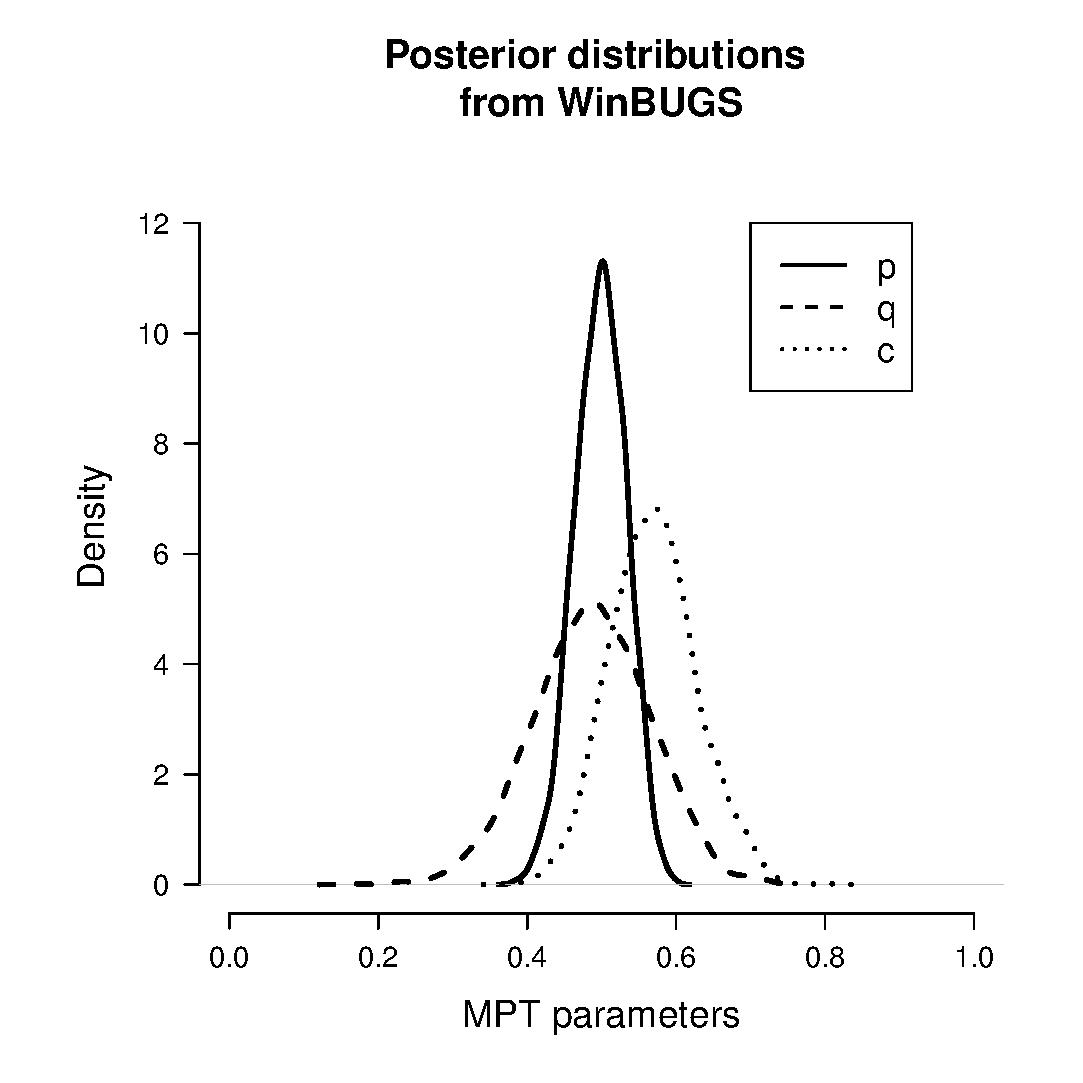
\includegraphics[width=0.485\textwidth]{figs/bi3_mpt_posteriors.eps}
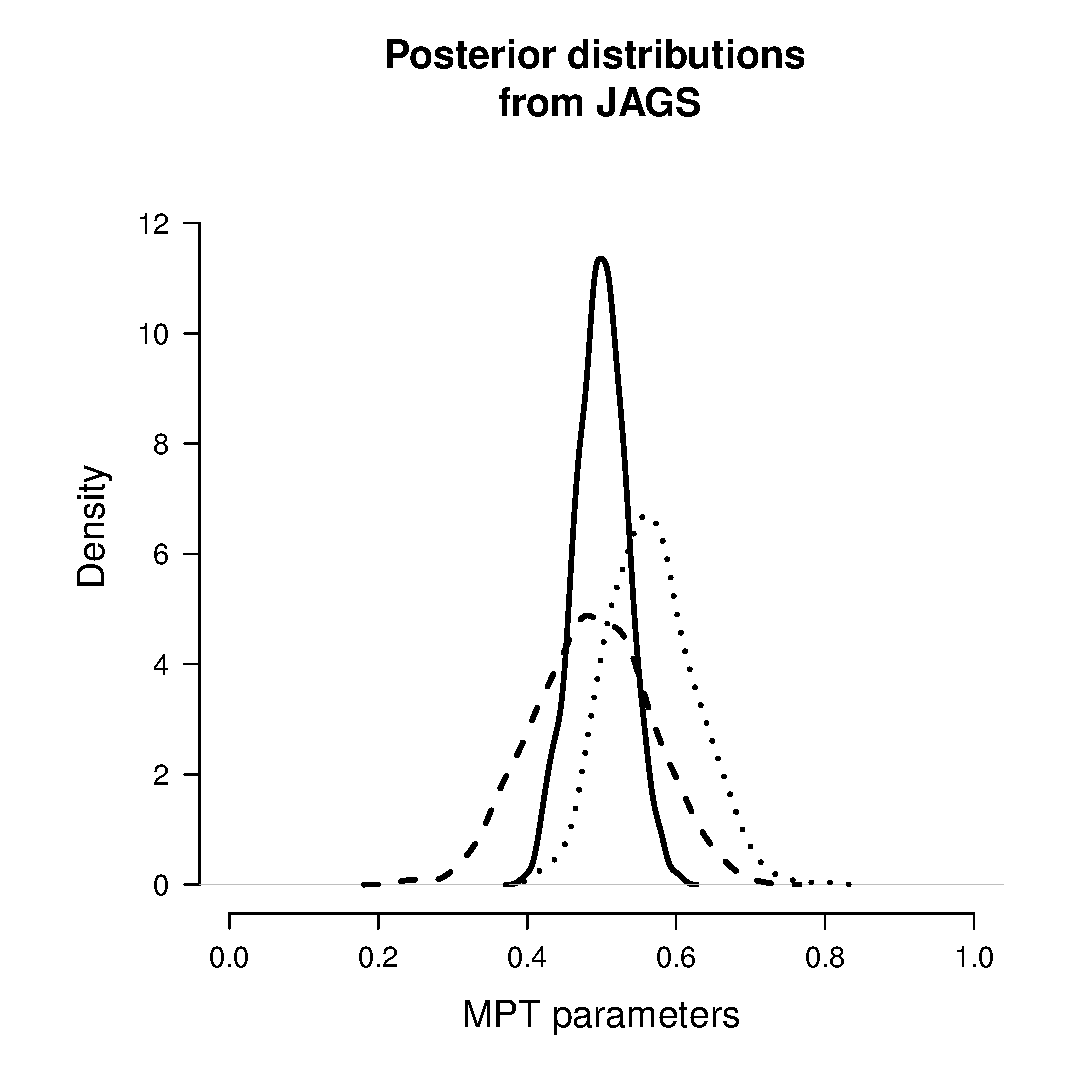
\includegraphics[width=0.485\textwidth]{figs/bi3_mpt_posteriors_jags.eps}
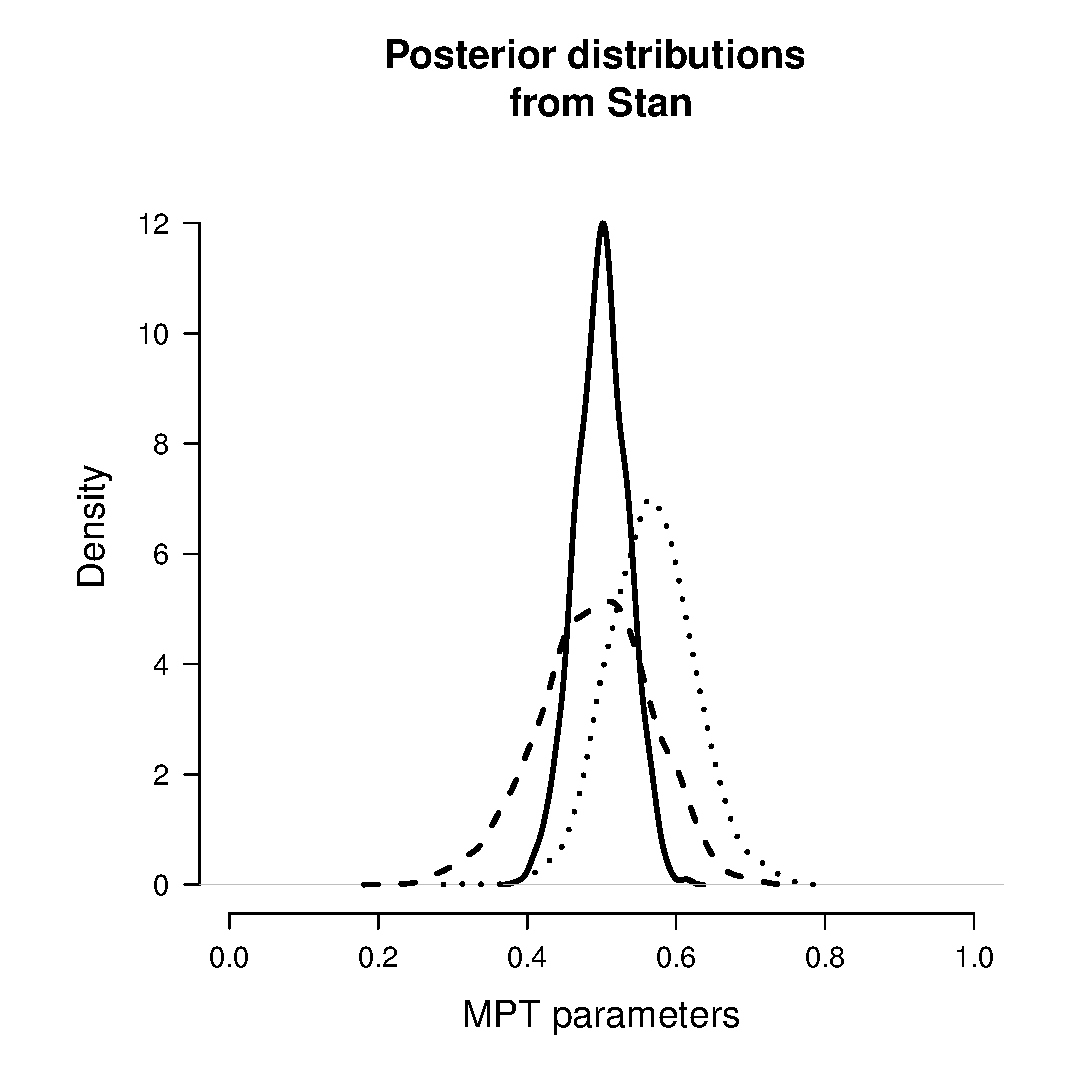
\includegraphics[width=0.485\textwidth]{figs/bi3_mpt_posteriors_stan.eps}
\caption{The posterior distribution of the parameters of the no--conflict MPT model obtained from WinBUGS, JAGS, and Stan in combination with R. The solid, dashed, and dotted lines show the posterior distribution of the $p$, $q$, and $c$ parameters, respectively.}\label{fig:bi3:mpt_post}
\end{figure*} 



\subsection{Working from R using R2jags}

The JAGS code for the generative specification of the no--conflict model is identical to the WinBUGS code presented in the previous section, and so is the R code for creating the data and generating the initial values. Once the \code{R2jags} package is loaded by typing \code{library(R2jags)}, the following R code can be used to call JAGS and sample from the posterior distribution of the parameters:

\begin{lstlisting}
samples <- jags(data=mydata,inits=myinits,parameters.to.save=myparameters,
    model.file ="noconflict.txt", 
    n.chains=3, n.iter=3500, n.burnin=500, n.thin=5, DIC=FALSE)
\end{lstlisting}

\noindent JAGS returns the posterior samples for the three model parameters in the \code{samples} object. The posterior distribution of the parameters is shown in the second column of Figure~\ref{fig:bi3:mpt_post}. The posteriors obtained with JAGS are essentially indistinguishable from the ones obtained with WinBUGS.



\subsection{Working from R using rstan}

The Stan code for the non--conflict model again differs somewhat from the {WinBUGS/JAGS} code:

\begin{lstlisting}
data{
    int cons[4];
    int inco[4];
    int neut[4];
}
parameters{
    real<lower=0,upper=1> p;
    real<lower=0,upper=1> q;
    real<lower=0,upper=1> c;
}
transformed parameters{
    real<lower=0,upper=1> pq;
    real<lower=0,upper=1> pc;
    simplex[4] theta1;
    simplex[4] theta2;
    simplex[4] theta3;

    pq <- p * q;
    pc <- p * c;

    // consistent condition
    theta1[1] <- ( 1 + p + q - pq + 4 * pc ) / 6;  // Eq. (*@\ref{eq:mpt10}@*)
    theta1[2] <- ( 1 + p + q - pq - 2 * pc ) / 3;  // Eq. (*@\ref{eq:mpt11}@*)
    theta1[3] <- ( 1 - p - q + pq ) / 6;           // Eq. (*@\ref{eq:mpt12}@*)
    theta1[4] <- ( 1 - p - q + pq ) / 3;           // Eq. (*@\ref{eq:mpt13}@*)
	
    // inconsistent condition
    theta2[1] <- ( 1 + p - q + pq + 4 * pc ) / 6;  // Eq. (*@\ref{eq:mpt14}@*)
    theta2[2] <- ( 1 + p - q + pq - 2 * pc ) / 3;  // Eq. (*@\ref{eq:mpt15}@*)
    theta2[3] <- ( 1 - p + q - pq ) / 6;           // Eq. (*@\ref{eq:mpt16}@*)
    theta2[4] <- ( 1 - p + q - pq ) / 3;           // Eq. (*@\ref{eq:mpt17}@*)
	
    // neutral condition
    theta3[1] <- ( 1 + p + 4 * pc ) / 6;           // Eq. (*@\ref{eq:mpt18}@*)
    theta3[2] <- ( 1 + p - 2 * pc ) / 3;           // Eq. (*@\ref{eq:mpt19}@*)
    theta3[3] <- ( 1 - p ) / 6;                    // Eq. (*@\ref{eq:mpt20}@*)
    theta3[4] <- ( 1 - p ) / 3;                    // Eq. (*@\ref{eq:mpt21}@*)
}
model{
    // priors
    p ~ beta(1,1);                                 // Eq. (*@\ref{eq:mpt22}@*)
    q ~ beta(1,1);                                 // Eq. (*@\ref{eq:mpt23}@*)
    c ~ beta(1,1);                                 // Eq. (*@\ref{eq:mpt24}@*)
    cons ~ multinomial(theta1);                    // Eq. (*@\ref{eq:mpt7}@*)
    inco ~ multinomial(theta2);                    // Eq. (*@\ref{eq:mpt8}@*)
    neut ~ multinomial(theta3);                    // Eq. (*@\ref{eq:mpt9}@*)
}
\end{lstlisting}

Once the model specification is saved as \file{noconflict.stan}, the \code{rstan} package has been loaded by typing \code{library(rstan)}, and R objects have been created that contain the data, initial values, and parameters of interest, the following code can be used to obtain samples from the posterior distributions of the parameters:

\begin{lstlisting}
samples <- stan(data = mydata, init = myinits, pars = myparameters,
	file = 'noconflict.stan',
	chains = 3, iter = 3500, warmup = 500, thin = 5)
\end{lstlisting}

\noindent The posterior samples for the three model parameters are returned in the \code{samples} object. The third column of Figure \ref{fig:bi3:mpt_post} shows estimates of the posterior densities based on the sampled values; the posteriors closely resemble those obtained with WinBUGS and JAGS.



\subsection{Working from MATLAB using Trinity}
The code to fit the no--conflict model from MATLAB using Trinity is again very formulaic, and differs very little between the three computational engines. In the bare--bones script automatically generated by \code{trinity new}, we first enter the data:
\begin{lstlisting}
cons = [  78 ,  70 ,   7 ,  15 ] ;
inco = [ 102 ,  55 ,  40 ,  53 ] ;
neut = [  63 ,  45 ,  13 ,  21 ] ;
N = [sum(cons) sum(inco) sum(neut)];
\end{lstlisting}

After the data are entered, the model definition needs to be provided as a cell string. We omit the model specification here because both the {WinBUGS/JAGS} and Stan versions are fully given in the previous sections.

Next, we list the parameters of interest in a cell variable:
\begin{lstlisting}
parameters = {
    'c' 'p' 'q'
    };
\end{lstlisting}
\noindent and we write a function that generates a structure containing one random value for each parameter in a field:
\begin{lstlisting}
generator = @()struct(...
    'c', rand, ...
    'p', rand, ...
    'q', rand  ...
    );
\end{lstlisting}
We also enter the data into a structure where we match the names of the fields to the variable names in the model definition:
\begin{lstlisting}
data = struct(...
    'cons', cons, ...
    'inco', inco, ...
    'neut', neut, ...
    'N'   , N     ...
    );
\end{lstlisting}
After selecting an engine, the \code{callbayes} function is called with mostly default settings:
\begin{lstlisting}
%% Run Trinity with the CALLBAYES() function
tic
[stats, chains, diagnostics, info] = callbayes(engine, ...
    'model'          ,     model , ...
    'data'           ,      data , ...
    'outputname'     , 'samples' , ...
    'init'           , generator , ...
    'modelfilename'  ,   proj_id , ...
    'datafilename'   ,   proj_id , ...
    'initfilename'   ,   proj_id , ...
    'scriptfilename' ,   proj_id , ...
    'logfilename'    ,   proj_id , ...
    'nchains'        ,        4  , ...
    'nburnin'        ,      1e4  , ...
    'nsamples'       ,      1e4  , ...
    'monitorparams'  ,   parameters  , ...
    'thin'           ,        5  , ...
    'refresh'        ,     1000  , ...
    'workingdir'     ,    ['/tmp/' proj_id]  , ...
    'verbosity'      ,        0  , ...
    'saveoutput'     ,     true  , ...
    'parallel'       ,  isunix() , ...
    'modules'        ,  {'dic'}  );
\end{lstlisting}

The engine will return, among others, the \code{chains} variable containing posterior samples for all three parameters of interest. We can inspect the results, and we can use the \code{codatable} function to give qualitative feedback about the convergence of the MC chains:  
\begin{lstlisting}
if any(codatable(chains, @gelmanrubin) > 1.1)
    grtable(chains, 1.1)
    warning('Some chains were not converged!')
else
    disp('Convergence looks good.')
end
\end{lstlisting}

Finally, we can inspect the posterior means by chain using the \code{stats} structure:
\begin{lstlisting}
disp('Posterior means by chain:')
disp(stats.mean)
\end{lstlisting}
\noindent as well as check some basic descriptive statistics averaged over all chains:
\begin{lstlisting}
disp('Descriptive statistics for all chains:')
codatable(chains)
\end{lstlisting}
\noindent and visually inspect the posterior distributions using the \code{smhist} function:
\begin{lstlisting}
smhist(chains, '^c$|^q$|^p$');
\end{lstlisting}
\noindent where the regular expression may be read as ``match only variables whose name is exactly \code{c} or exactly \code{q} or exactly \code{p}''.
The output of the last command---the posterior distribution of the parameters---is shown in Figure~\ref{fig:bi3:posteriorsTrinity}.

\begin{figure}[bt] \centering
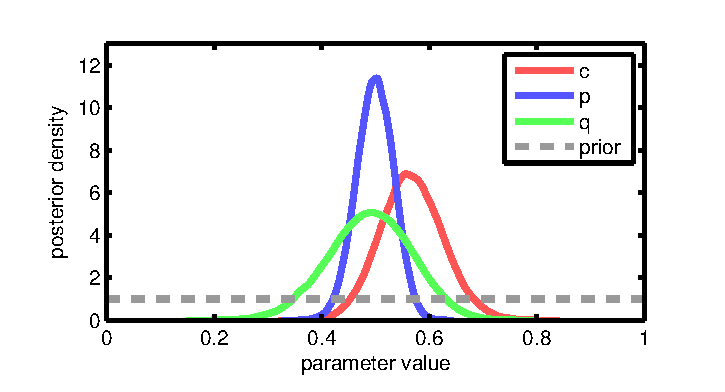
\includegraphics[%viewport=145 295 475 485, clip=true,
scale=0.9]{figs/bi3_posteriors}
\caption{{The posterior distribution of the parameters of the no--conflict MPT model obtained from JAGS in combination with Trinity.}}\label{fig:bi3:posteriorsTrinity}
\end{figure}

\subsubsection{Testing hypotheses} 
After the posterior samples have been drawn, and posterior distributions possibly visualized as above, there remains the issue of testing hypotheses relating to parameters. With the current false--memory data set, one hypothesis of interest might be that the probability $p$ of encoding the traffic light is greater (versus lower) than chance (Hypothesis~1). The same question might be asked of the probability $c$ of encoding the light color (Hypothesis~2).

Given samples from the posterior, a convenient way of computing the posterior probability that a hypothesis is true is by computing the proportion of posterior samples in which the hypothesis holds. To test Hypothesis~1, we would calculate the proportion of cases in which $p > 0.5$. To test Hypothesis~2, we calculate the proportion of cases in which $c > 0.5$.

The \code{codatable} command is useful in this regard. Custom statistics on the posterior samples can be computed by providing anonymous functions as secondary input variables. A quick way of counting the proportion of cases in which a condition is true is to make use of the fact that MATLAB represents logically true statements as $1$ and false statements as $0$. Hence, the anonymous function \code{@(x)mean(x>.5)} will return the proportion of cases where the input is greater than $0.5$:

\begin{lstlisting}
>> codatable(chains, '^c$|^p$', @mean, @(x)mean(x>.5))
  Estimand        mean  @(x)mean(x>.5)
         c       0.558          0.8441
         p      0.4956          0.4547
\end{lstlisting}
As it turns out, the probability of Hypothesis~1 given the data is about 84\% and that of Hypothesis~2 is about 45\%. In other words, neither of the hypotheses is strongly supported by the data. In fact, as Figure~\ref{fig:bi3:posteriorsTrinity} shows, most of the posterior mass is clustered near $0.5$ for all parameters.

\section{Conclusion}

{Bayesian methods are rapidly rising from obscurity and into the mainstream of psychological science. While {Bayesian equivalents of} many standard analyses, such as the $t$ test and linear regression, can be conducted in off--the-shelf software such as JASP \cite{jasp}, custom models will continue to require a flexible programming framework and, unavoidably, some degree of software MacGyverism. To implement specialized models, researchers may write their own MCMC samplers, a process that is time--consuming and labor--intensive, and does not come easy to investigators untrained in computational methods. Luckily, general--purpose MCMC engines---such as WinBUGS, JAGS, and Stan---provide easy--to--use alternatives to custom MCMC samplers. These software packages hit the sweet spot for most psychologists; they provide a large degree of flexibility at a relatively low {time} cost.} 

{In this tutorial, we demonstrated the use of three popular Bayesian software packages in conjunction with two scientific programming languages, R and MATLAB. This combination allows researchers to implement custom Bayesian analyses from already familiar environments. As we illustrated, models as common as a linear regression can be easily implemented in this framework, but so can more complex models, such as multinomial processing trees (MPT; \citeNP{BatchelderRiefer1980, Chechile1973, riefer1988multinomial}).} 

{Although the tutorial focused exclusively on non--hierarchical models, the packages may also be used for modeling hierarchical data structures (e.g, \citeNP{Lee2011Hier}). In hierarchical modeling, rather than estimating parameters separately for each unit (e.g., participant), we model the between--unit variability of the parameters with group--level distributions. The group--level distributions are used as priors to ``shrink'' extreme and poorly constrained estimates to more moderate values. Hierarchical estimation can provide more precise and less variable estimates than non--hierarchical estimation, especially in data sets with relatively few observations per unit \cite{FarrellLudwig2008,RouderEtAl2005}. Hierarchical modeling is rapidly gaining popularity in psychology, largely by virtue of to the availability of accessible MCMC packages. The WinBUGS, JAGS, and Stan implementation of most hierarchical extensions is very straightforward and often does not require more than a few additional lines of code. For the hierarchical WinBUGS implementation of regression models, the reader is referred to \citeA{GelmanHill2007}. For the hierarchical implementation of custom models, such as multinomial processing trees, signal detection, or various response time models, the reader is referred to \citeA{LeeWagenmakersBayesBook}, \citeA{MatzkeEtAlPsychometrika}, \citeA{matzkewagenmakers2009}, \citeA{NilssonEtAl2011}, \citeA{RouderEtAl2008PDP} and \citeA{VandekerckhoveEtAl2011}.}

{Although the goal of our tutorial was to demonstrate the use of general--purpose MCMC software for Bayesian \textit{parameter estimation}, our MPT--example has also touched on Bayesian hypothesis testing. Various other Bayesian methods are available that rely on MCMC--output to test hypotheses and formally compare the relative predictive performance of competing models. For instance, \citeA{WagenmakersEtAl2010SDPsychologists} and \citeA{WetzelsEtAl2009PBR} discuss the use of the Savage--Dickey density ratio, a simple procedure that enables researchers to compute Bayes factors \cite{Jeffreys1961,KassRaftery1995} for nested model comparison using the height of the prior and posterior distributions obtained from WinBUGS. \citeA{Vandekerckhove2015} shows how to use posterior distributions obtained from WinBUGS and JAGS to compute Bayes factors for non--nested MPTs using importance sampling. \citeA{LodewyckxEtAl2011tutorial} outline a WinBUGS implementation of the product--space method, a transdimensional MCMC approach for computing Bayes factors for nested and non--nested models}. Most recently, \citeA{gronau2017tutorial} provide a tutorial on bridge sampling---a new, potentially very powerful method that is under active development.  It is important to note, however, that all of these methods are almost all quite difficult to use and can be unstable, especially for high-dimensional problems.

{Throughout the tutorial, we have advocated WinBUGS, JAGS, and Stan as flexible and user-friendly alternatives to homegrown sampling routines. Although the MCMC samplers implemented in these packages work well for the majority of models used in psychology, they may be inefficient and impractical for some. For instance, models of choice and response times, such as the linear ballistic accumulator \cite{BrownHeathcote2008LBA} or the lognormal race \cite{rouder2015lognormal}, are notoriously difficult to sample from using standard MCMC software. In these cases, custom-made MCMC routines may be the only solution. For examples of custom-made and non--standard MCMC samplers, the reader is referred to \citeA{RouderLu2005} and \citeA{turner2013method}, respectively.}

{Their general usefulness notwithstanding, the three packages all have their own set of limitations and weaknesses. WinBUGS, as the name suggests, was developed specifically for Windows operating systems. Although it is possible to run WinBUGS under OS X and Linux using emulators such as Darwine and CrossOver or compatibility layers such as Wine, user experience is often jarring. Even under Windows, software installation is a circuitous process and requires users to decode a registration key and an upgrade patch via the GUI. Once installed, users typically find the GUI inflexible and labor--intensive. In interaction with R, user experience is typically more positive. Complaints focus mostly on WinBUGS' cryptic error messages and the limited number of built--in functions and distributions. Although the WinBUGS Development Interface (WBDev; \citeNP{Lunn2003}) enables users to implement custom--made functions and distributions, it requires experience with Component Pascal and is poorly documented. \citeA{MatzkeEtAlJEPGen} provide WBDev scripts for the truncated--normal and ex--Gaussian distributions; \citeA{wetzels2010bayesian} provide an excellent WBDev tutorial for psychologists, including a WBDev script for the shifted--Wald distribution. Importantly, the BUGS Project has shifted development away from WinBUGS; development now focuses on OpenBUGS (\url{http://www.openbugs.net/w/FrontPage}).}

{Stan comes equipped with interfaces to various programming languages, including R, Python and MATLAB, and only requires the installation of the specific interface package, which is easy and straightforward under most common operating systems. In terms of computing time, Stan seems a particularly suitable choice for complex models with many parameters and large posterior sample sizes. This advantage in computing time is due to the fact that Stan compiles the sampling model to a \code{C++} program before carrying out the sampling process. The downside of this compilation step is that, particularly for small models as used in the present tutorial, compilation of the model might require more time than the sampling process itself, in which case WinBUGS or JAGS seem a more advantageous choice.}

{Finally, we will highlight two advantages of JAGS over Stan. First, as illustrated in our example code, Stan code requires variable declaration and as a result can be somewhat more complicated than JAGS code. Second, as a consequence of Stan's highly efficient Hamiltonian Monte Carlo sampling algorithm, some model specifications are not allowed---in particular, Stan does not easily allow model specifications that require inference on discrete parameters, which reduces its usefulness if the goal is model selection rather than parameter estimation.}

{We demonstrated the use of three popular Bayesian software packages that enable researchers to estimate parameters in a broad class of models that are commonly used in psychological research. We focused on WinBUGS, JAGS, and Stan, and showed how they can be interfaced from R and MATLAB. We hope that this tutorial can serve to further lower the threshold to Bayesian modeling for psychological science.}

\bibliographystyle{apacite}
\bibliography{bi3}
